In questo capitolo vengono esposti i concetti alla base del progetto CAMUS. In questo modo viene fornito al lettore un quadro generale delle tematiche che verranno affrontate nei successivi capitoli. Il capitolo inizia con l'introduzione del concetto di \emph{context awareness}, che è la prima delle due anime del progetto, seguita dalla presentazione del modello del contesto che viene utilizzato in CAMUS, il \emph{Context Dimension Tree}. Successivamente viene presentato il secondo pilastro del progetto, i \emph{mashup}, e in particolar modo la tipologia di nostro interesse, i \emph{mobile mashup}. Di seguito verranno analizzate le varie tipologie di \emph{servizi} che il web mette a disposizione. La loro posizione non deve trarre in inganno: i servizi sono egualmente importanti in quanto permettono all'intero sistema di funzionare: infatti forniscono le informazioni che vengono presentate all'utente; senza servizi l'intero progetto non sarebbe altro che un'impalcatura fine a se stessa. Viene inoltre fornita una panoramica sulle tecnologie e framework utilizzati per sviluppare il backend di CAMUS ed in seguito per quanto riguarda lo sviluppo \emph{Cross-Platform} e le tecnologie sfruttate per l'app mobile. Infine viene effettuato un confronto con i principali competitor di CAMUS, cioè tutti i lavori esistenti che affrontano le medesime tematiche.

\section{Context-Awareness\label{sec:context-awareness}}

Il concetto di \emph{contesto} viene citato in diverse aree di ricerca, come la filosofia, la psicologia e l'informatica. Il \emph{contesto} gioca spesso un ruolo importante nel definire un comportamento o l'interpretazione dell'ambiente; dei cambiamenti nel contesto possono cambiare la percezione del momento che si sta vivendo. La parola \virgolette{contesto} deriva dalle parole latine \emph{con} e \emph{texere}, che significa tessere intrecciate, intrecciare. Viene definito come \virgolette{il complesso delle circostanze e delle situazioni nelle quali un fatto o un fenomeno si verificano}\footnote{Dizionario Garzanti: \url{http://www.garzantilinguistica.it/ricerca/?q=contesto}}.

In informatica il concetto di \emph{contesto} è riferito all'idea che i computer possano avere una percezione dell'ambiente e che riescano dunque a modificare il loro comportamento in base alla situazione. I dispositivi devono dunque acquisire informazioni relative all'ambiente in cui operano e tramite determinate regole, che possono essere sia staticamente fissate che dinamicamente dedotte tramite algoritmi di intelligenza artificiale, devono reagire di conseguenza, utilizzando la strategia più idonea alla situazione corrente. Il termine \emph{context awareness} è stato introdotto per la prima volta in ambito informatico a opera di Schilit \cite{schilit1994context}\cite{schilit1994disseminating}.

Agli albori il \emph{contesto} veniva inteso solamente come la posizione nella quale si trova l'utente, come discusso da Dey in \cite{dey2001understanding}; negli ultimi anni invece si è iniziato a pensare al \emph{contesto} non solo come uno stato, bensì come un processo più vasto che coinvolge diversi aspetti relativi all'utente. Sono stati dunque ideati modelli di \emph{contesto} sofisticati e generali, in modo che possano adattarsi a diverse situazioni d'utilizzo \cite{DBLP:journals/sigmod/BolchiniCQST07} \cite{baldauf2007survey}.

In particolare il \emph{contesto} viene utilizzato per realizzare applicazioni che siano in grado di \emph{a)} adattare l'interfaccia grafica, \emph{b)} filtrare l'insieme dei dati che sono realmente rilevanti, \emph{c)} migliorare la precisione dei dati raccolti, \emph{d)} scoprire servizi, \emph{e)} predirre alcune scelte dell'utente o \emph{f)} realizzare ambienti \emph{intelligenti}.

Si prenda come esempio un dispositivo mobile fornito ai visitatori di un museo di storia naturale che sfrutti il contesto per \emph{a)} adattare la struttura e l'aspetto dell'interfaccia grafica in base alle caratteristiche del visitatore, sia esso una persona con problemi di vista oppure un bambino; \emph{b)} mostrare informazioni diverse in base agli interessi del visitatore (es.: geologia, paleontologia, ecc.) oppure in base alla stanza in cui si trova; \emph{c)} imparare dalle precedenti scelte effettuate dall'utente quali potranno essere le informazioni di maggiore gradimento; \emph{d)} proporre al visitatore determinati servizi, come l'acquisto dei biglietti per una mostra temporanea o la prenotazione di un posto nello spettacolo sui dinosauri che sta per incominciare nella sala adiacente; \emph{e)} conoscere la posizione del visitatore in base ai sensori che monitorano l'ambiente; \emph{f)} fornire dei contenuti attivi al visitatore su cosa accade in un particolare ambiente.

I sistemi \emph{context aware} riguardano l'\emph{acquisizione} del contesto (per esempio tramite l'utilizzo di determinati sensori), l'\emph{astrazione} e il \emph{riconoscimento} del contesto (per esempio associare un determinato stimolo al contesto) e il \emph{comportamento} adatto alla situazione riconosciuta (per esempio l'esecuzione di un'azione innescata dal contesto) \cite{schmidt2003ubiquitous}. L'utilizzo del \emph{contesto} permette la realizzazione di interfacce grafiche innovative e viene spesso utilizzato nella \emph{computazione ubiqua} e nei \emph{dispositivi indossabili}.

Nella seguente sezione verrà presentato nel dettaglio il \emph{Context Dimension Tree}, un modello di contesto che sfrutta una struttura ad albero per descrivere la situazione nel quale si trova l'utente. Tra la moltitudine di alternative esistenti viene presentato questo modello in particolare perchè è quello che verrà utilizzato nel progetto CAMUS, quindi la comprensione della sua rappresentazione e delle potenzialità saranno utili per i successivi capitoli.

\subsection{Context Dimension Tree\label{sec:context-dimension-model}}

In questa sezione viene presentato nel dettaglio il \emph{Context Dimension Tree} \cite{DBLP:journals/is/BolchiniQT13}, in quanto è il modello di rappresentazione del contesto che è stato selezionato per l'utilizzo nel progetto CAMUS. Nel \emph{Context Dimension Tree} il contesto viene rappresentato come un albero $\mathcal{T} = {<}N, E, r{>} $, che descrive i possibili contesti nei quali ci si può trovare in una data situazione. \`E formato da una radice \emph{r}, un insieme di nodi \emph{N}, che vengono partizionati nei sottoinsiemi dei \emph{nodi dimensione} $N_D$, colorati di nero, e nei \emph{nodi concetto} $N_C$, colorati di bianco, che rappresentano i possibili valori che possono assumere le dimensioni, e dall'insieme dei collegamenti tra i nodi \emph{E}. La radice \emph{r} è un \emph{nodo concetto}, in quanto rappresenta il contesto più generale possibile, che corrisponde dunque all'intero dataset.

\begin{figure}[ht]
	\centering
	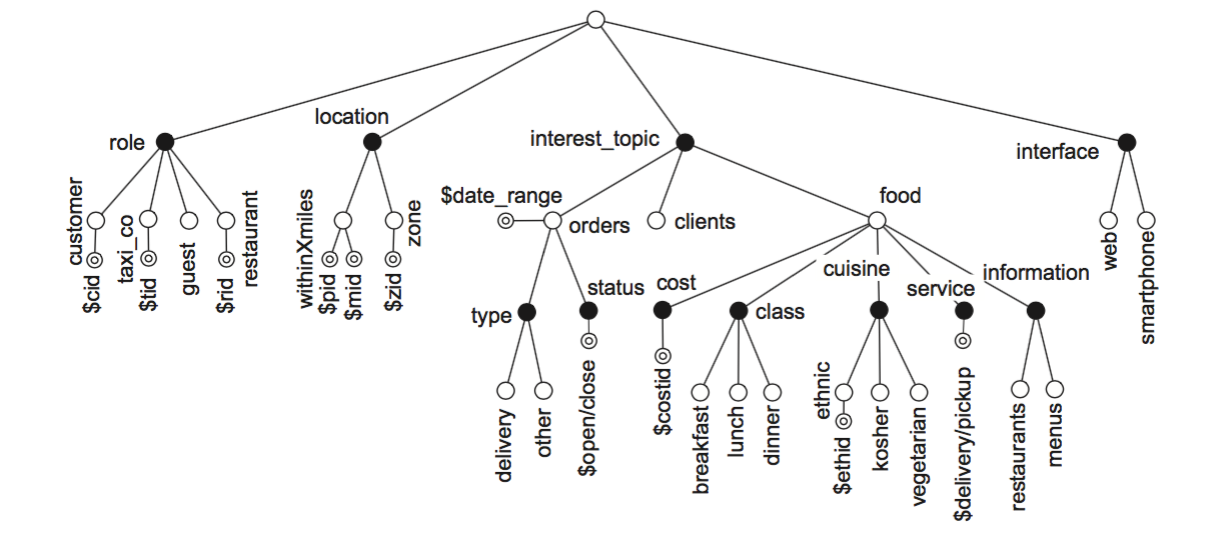
\includegraphics[width=\textwidth]{2-nozioni-preliminari/Immagini/esempio_cdt.png}
	\caption[Context Dimension Tree]{Context Dimension Tree (Fonte: \virgolette{CARVE: context-aware automatic view de nition over relational databases}, 2013)}\label{fig:context-dimension-tree}
\end{figure}

Le dimensioni che sono dirette discendenti della radice vengono chiamate \emph{dimensioni principali}, perché definiscono le differenti caratteristiche dell'utente e del contesto nel quale agiscono. Nell'esempio in Figura \ref{fig:context-dimension-tree}, le \emph{dimensioni principali} sono il \emph{ruolo} dell'utente, l'\emph{interfaccia} tramite la quale accede ai dati, l'\emph{interest topic} e la \emph{posizione} in cui si trova. Inoltre, ogni valore può essere ulteriormente specializzato tramite \emph{sottodimensioni}, che a loro volta formano un sottoalbero. Per esempio, l'interest topic \virgolette{ordine} può essere analizzato in base allo \emph{stato} in cui si trova oppure in base alla sua \emph{tipologia}.

Ogni nodo del CDT è caratterizzato dalla sua tipologia, che può essere \emph{dimensione} o \emph{concetto}, e dalla sua etichetta; può essere identificato univocamente tramite l'unico percorso che lo collega fino alla radice. Senza perdita di generalità, viene adottata l'ipotesi che ogni etichetta sia unica in un albero, quindi ogni nodo può essere identificato semplicemente dalla sua etichetta. I collegamenti tra i vari nodi non vengono invece etichettati.

L'alternanza tra nodi \emph{dimensione} e \emph{concetto} fa sì che vengano create delle \emph{generazioni}, ognuna delle quali sarà formata da nodi dello stesso colore, e ogni colore verrà alternato man mano che si prosegue discendendo nell'albero: dunque ogni \emph{nodo dimensione} può avere come figli solo nodi di tipo \emph{concetto} e viceversa.

\`E inoltre possibile associare uno o più \emph{parametri} ai nodi concetto e ai nodi dimensione che sono foglie dell'albero. Ogni parametro permette di raffinare ulteriormente la selezione dei dati e selezionare un sottoinsieme del dataset particolare. Per esempio, il parametro \virgolette{intervallo} associato al concetto \emph{ordini} permette di indicare un intervallo di date e quindi di selezionare esclusivamente gli ordini che sono riferiti alle date indicate.

Per ogni \emph{nodo dimensione} è possibile selezionare al massimo un nodo concetto tra i suoi figli oppure, se non possiede alcun nodo figlio, deve essere selezionato obbligatoriamente uno e un solo parametro. L'utilizzo dei \emph{parametri} aumenta il potere espressivo del modello, in quanto lo rende più semplice per l'utilizzo da parte del designer. Si è resa necessaria l'introduzione dei parametri in quanto non tutti i concetti espressi da una dimensione possono essere enumerati. Per esempio, la dimensione \virgolette{costo} può assumere infiniti valori ed è quindi più appropriato l'utilizzo di un parametro che sia variabile.

Ora che è stato definito il modello è necessario spiegare come viene rappresentato uno specifico \emph{contesto}. Dato un \emph{Context Dimension Tree} $\mathcal{T} = {<}N, E, r{>} $, un \emph{contesto} è definito dalla grammatica in Figura \ref{fig:grammatica-cdt} con assioma \emph{context}.

\begin{figure}[ht]
	\begin{equation*}
	C =
	\begin{cases}
		{<}context{>} \leftarrow {<}context\_element{>}\ |\ {<}context\_element{>} \land {<}context{>}\\
		{<}context\_element{>} \leftarrow dim\_name: {<}value\_item{>}\ |\ dim\_name\ ({<}parameter{>})\\
		{<}value\_item{>} \leftarrow value\ |\ value\ ({<}parameters{>})\\
		{<}parameters{>} \leftarrow {<}parameters{>} \land {<}parameter{>}\ |\ {<}parameter{>}\\
		{<}parameter{>} \leftarrow param\_name: param\_value
	\end{cases}
	\end{equation*}
	\caption{Grammatica del Context Dimension Tree}\label{fig:grammatica-cdt}
\end{figure}

Un \emph{contesto} è formato dalla congiunzione tra uno o più \emph{elementi del contesto}. Ogni elemento del contesto è formato dal nome della dimensione seguita da uno dei valori scelto tra i nodi che sono suoi figli diretti, oppure dal valore che assume l'unico parametro a essa associato, nel caso in cui la dimensione è una foglia dell'albero. Ogni valore può essere a sua volta raffinato aggiungendo il/i parametro/i a esso associati.

Non è necessario selezionare per forza tutte le dimensioni presenti nell'albero: non selezionare alcun valore relativo a una dimensione equivale a essere indifferenti rispetto quella particolare situazione. Ogni dimensione che non viene selezionata non influirà nel processo di acquisizione dei dati contestuali.

\begin{figure}[ht]
	\begin{align*}
		C =\ &role : customer\ (\$cid : ``Bill")\ \land \\
			&interest\_topic : orders\ \land \\
			&interface : smartphone
	\end{align*}
	\caption{Esempio di contesto}\label{fig:esempio-contesto-base}
\end{figure}

In Figura \ref{fig:esempio-contesto-base} viene mostrato un esempio che rappresenta il contesto in cui il cliente Bill è interessato nel ricevere informazioni sui propri ordini sullo smartphone. Il contesto \emph{C} è quindi composto da tre elementi del contesto.

Infine, dopo aver discusso del modello e di come vengono rappresentati i vari contesti, resta da definire come è possibile acquisire i dati che sono pertinenti a un determinato contesto. Come evidenziato in \cite{DBLP:journals/cacm/BolchiniCOQRST09}, esistono due strategie principali per definire le associazioni tra i contesti e la porzione di dati rilevanti per i vari contesti, chiamate \emph{configuration-based mapping} e \emph{value-based mapping}.

\begin{figure}[ht]
	\centering
	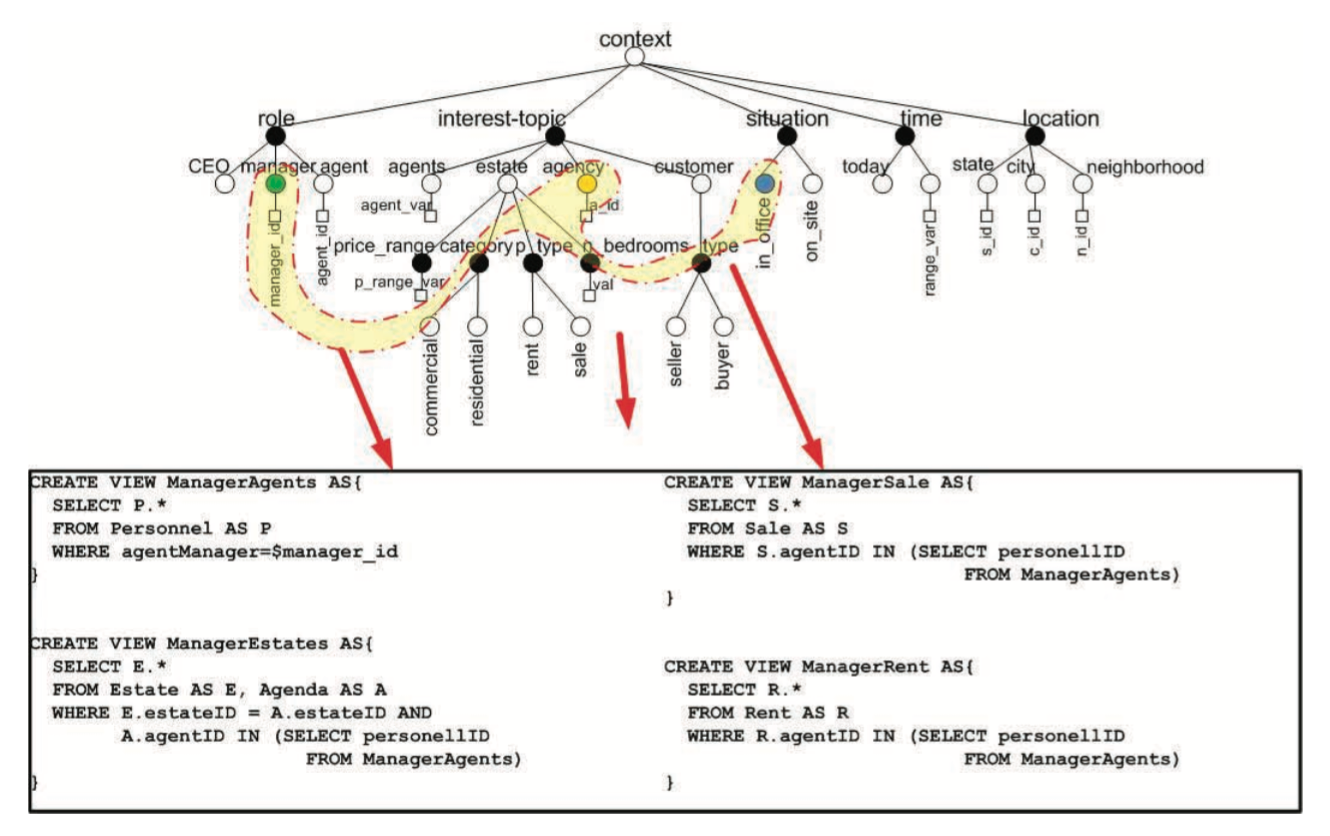
\includegraphics[width=\textwidth]{2-nozioni-preliminari/Immagini/configuration-based-mapping.png}
	\caption[Configuration-based mapping]{Configuration-based mapping (Fonte: \virgolette{And what can context do for data?}, 2009)}\label{fig:configuration-based-mapping}
\end{figure}

La strategia \emph{configuration-based mapping} prevede che il designer definisca per ogni contesto possibile la relativa porzione del dataset da mostrare. Questa operazione può essere effettuata definendo delle viste nel linguaggio specifico del database adottato. In Figura \ref{fig:configuration-based-mapping} viene mostrato un esempio per il contesto nel quale un manager è interessato alle informazioni relative le sue agenzie. In questo caso il designer specifica delle viste in linguaggio SQL relative al contesto specifico, mettendo in evidenza i dati del personale che lavora nelle agenzie gestite dal manager, i contratti di affitto e vendita e infine le informazioni relative alle proprietà.

Questa strategia ha il vantaggio di generare delle viste molto precise rispetto al contesto che vogliono rappresentare, ma ha l'enorme svantaggio che deve essere ripetuta per ognuno dei possibili contesti che, com'è facilmente intuibile, possono essere in quantità molto elevata. Inoltre, se in futuro dovesse essere aggiunta un'ulteriore dimensione, sarebbe necessario modificare le varie associazioni per includere la nuova dimensione.

\begin{figure}[ht]
	\centering
	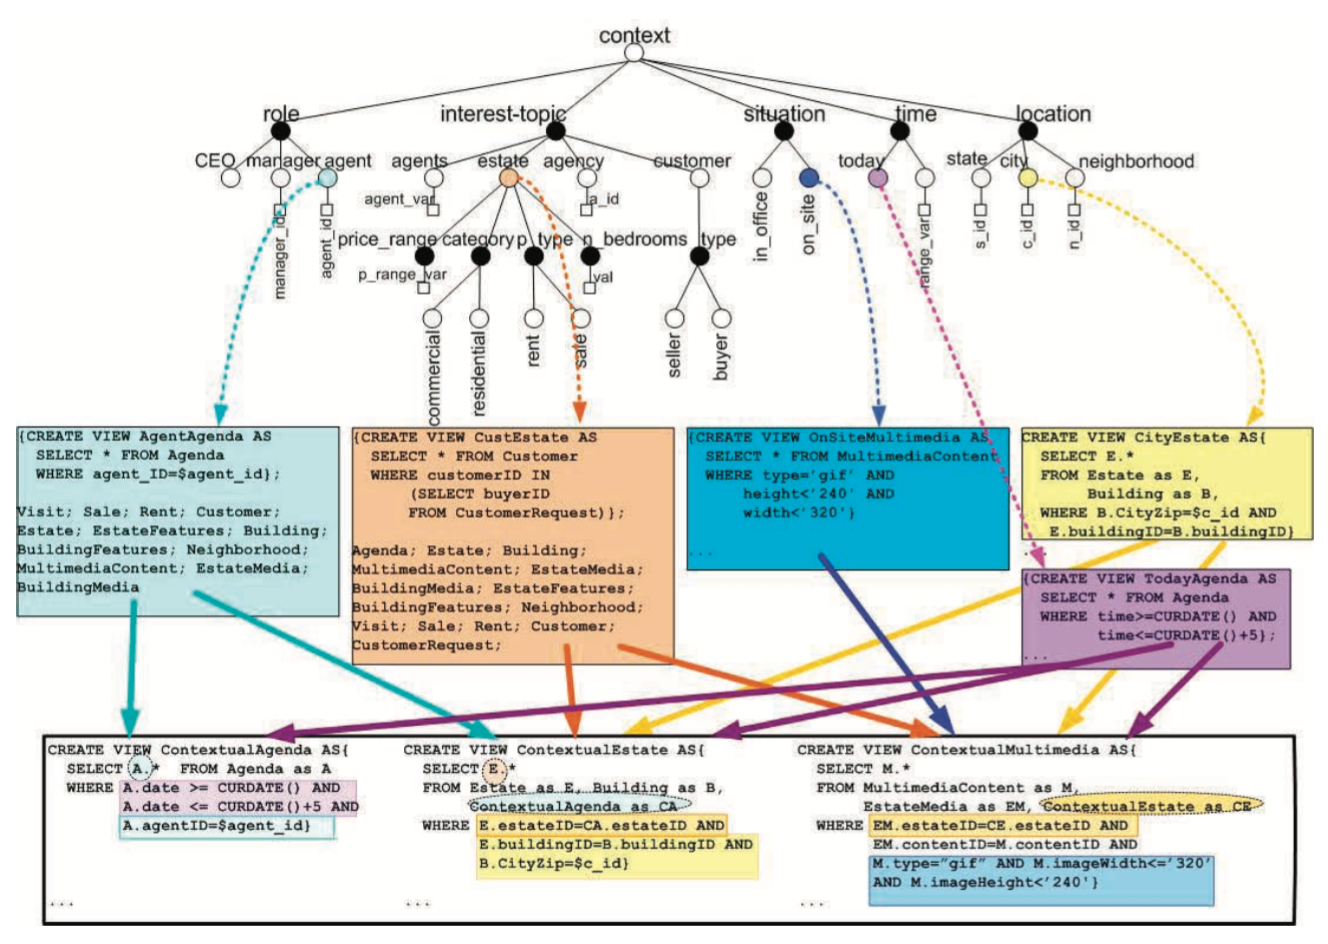
\includegraphics[width=\textwidth]{2-nozioni-preliminari/Immagini/value-based-mapping.png}
	\caption[Value-based mapping]{Value-based mapping (Fonte: \virgolette{And what can context do for data?}, 2009)}\label{fig:value-based-mapping}
\end{figure}

La strategia \emph{value-based mapping} permette di superare i limiti evidenziati per la strategia precedente. Questa strategia prevede che il designer definisca le viste parziali relative a un particolare elemento del contesto, indipendentemente dagli altri. Quindi, una volta selezionato un contesto, un algoritmo si occuperà di combinare assieme le varie viste parziali definite dai singoli elementi per formare la vista globale adatta allo specifico contesto. La Figura \ref{fig:value-based-mapping} mostra come il contesto dell'esempio precedente viene mappato tramite questa strategia. Le linee tratteggiate mostrano le viste parziali che vengono associate ai vari elementi del contesto, mentre nel riquadro in basso viene mostrata la vista globale generata dalla combinazione delle viste parziali. L'algoritmo di composizione delle view parziali è basato sull'utilizzo di diverse policy e operatori di composizione, tra i quali i più utilizzati sono \emph{double union}, \emph{double intersection} e \emph{double difference} \cite{DBLP:conf/er/BolchiniQR07}.

\section{Mashup\label{sec:mashup}}

In questa sezione vengono introdotti i \emph{Mashup}, la seconda anima del sistema CAMUS, e il loro ruolo nell'applicazione finale.
La parola \emph{Mashup}, che significa letteralmente miscuglio o combinazione, è un termine che può essere adottato in diversi ambiti.
Per esempio, in campo musicale, indicano due o più brani le cui tracce audio vengono tagliate e sovrapposte creando un nuovo brano. Un altro esempio è l'ambito dei contenuti video, dove due o più filmati sono montati in sequenza per ottenere un video dal significato diverso da quelli originali.
In informatica questo termine assume un significato simile, perché i mashup sono applicazioni che utilizzano contenuti e funzioni provenienti da due o più sorgenti\cite{DBLP:books/sp/DanielM14}.
Inizialmente la composizione era limitata all'utilizzo per la realizzazione rapida di siti web con contenuti di elevata dinamicità, vista la possibilità di integrare varie informazioni in modo molto intuitivo.

Molto diffuse in questa prima fase sono state le applicazioni che offrivano integrazione con mappe geografiche, come \emph{HousingMaps} \footnote{Housing Maps: \url{http://www.housingmaps.com}}, che combinava le informazioni tra Google Maps, per quanto riguarda ovviamente le mappe, e Craiglist, un portale che ospita annunci di diversa tipologia (es.: lavoro, incontri, ecc.).
%Altri esempi sono le mappe interattive che è possibile creare a partire da Google Maps o servizi simili; in questi casi viene arricchita la mappa con altre informazioni, a esempio traffico, dati demografici o altri dati. 

\begin{figure}[ht]
	\centering
	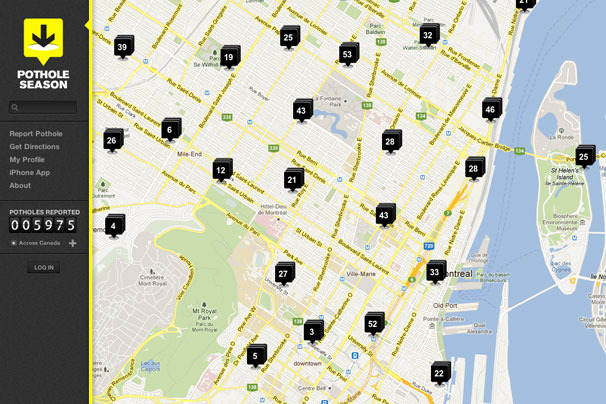
\includegraphics[width=\textwidth]{2-nozioni-preliminari/Immagini/potholes_service.jpg}
	\caption{Potholes Service}\label{fig:potholes}
\end{figure}

L'esempio in Figura \ref{fig:potholes} mostra un simpatico esempio di mashup che posiziona nella mappa le buche stradali segnalate dagli utenti presenti a Montreal in Canada, fornendo anche la possibilità di calcolare un itinerario per evitarle o almeno trovarne il meno possibile \footnote{Articolo con altri esempi: \url{http://www.pcworld.com/article/252243/top_10_cool_and_useful_google_maps_mashups.html}}. 

Con lo sviluppo dei social network e delle piattaforme di condivisione di contenuti multimediali, i mashup hanno assunto grande importanza perché è stato possibile creare nuove applicazioni utilizzando i metadati associati ai contenuti, arricchendo di informazioni il contenuto originale.
La diffusione dei mashup è presente anche in domini più critici, soprattutto per la facilità di creazione e la possibilità di essere utilizzati anche da utenti non esperti in ambito IT, di cui un esempio possono essere gli \emph{enterprise mashups}.
La crescita esponenziale della quantità di informazioni presente nel web, con i Big Data e il moltiplicarsi dei Web Service, ha portato i mashup a elemento fondamentale nella creazione delle applicazioni, per via della possibilità di filtrare i dati necessari all'utente finale e quindi rendere la visione di una parte significativa della moltitudine di informazioni provenienti dai servizi.

%Tra le diverse tipologie di mashups elencate in \cite{picozziTesiDottorato}, per quanto riguarda il progetto CAMUS, ci si soffermerà principalmente sui \emph{mobile mashups}.

\subsection{Classificazione dei mashup\label{sec:mashup-classification}}

I mashup possono essere distinti in diverse tipologie, a prescindere dalla piattaforma sulla quale vengono utilizzati.
In questo caso, la classificazione è basata soprattutto alla metodologia con la quale vengono integrate le diverse risorse che compongono i mashup. Vengono definite tre macro famiglie:

\begin{enumerate}
	\item \textbf{Consumer Mashups}
	Sono i mashup che combinano elementi visuali e dati da diverse fonti. Un ottimo esempio può essere considerato Housing Maps citato nella Sezione \ref{sec:mashup}, dove vengono integrati i dati provenienti da Craigslist e mostrati sulla mappa creata sfruttando le API di Google Maps
	\item \textbf{Data Mashups}
	Sono mashup che combinano più risorse di dati in una singola applicazione. Questa tipologia di mashup viene invece sfruttata per realizzare molte applicazioni, anche in settori di utilizzo diversi tra loro.
	Nell'ambito dei viaggi, un esempio viene fornito da Kayak \footnote{Kayak : \url{http://www.kayak.com}}, che è un sito di ricerca dei viaggi che acquisisce dati da oltre 100 siti diversi. Inoltre non vende direttamente i contenuti ai fornitori, ma si propone come un portale attraverso il quale i clienti possono essere dirottati verso le agenzie viaggi per completare la procedura di acquisto o specificare alcune esigenze particolari.
	Un altro ambito completamente differente riguarda Facile.it \footnote{Facile.it : \url{http://www.facile.it}}, che permette di confrontare diverse offerte per quanto riguarda diversi settori (es.: assicurazioni, mutui, linee telefoniche, ecc.), permettendo di visualizzarli in unico portale e valutare la proposta migliore per le esigenze dell'utente
	\item \textbf{Business Mashups}
	I business mashups sono utili per quanto riguarda l'in\-te\-gra\-zio\-ne di servizi business, permettendo di sviluppare più facilmente servizi integrati e, di conseguenza, semplificare l'utilizzo all'utente attraverso interfacce web. Si differiscono dai \emph{consumer mashup} a livello di integrazione con i sistemi business, perché sono necessarie funzionalità aggiuntive, riguardanti sicurezza, controllo di accesso, governance e complessità degli editor utilizzati. Un'altra differenza è data dall'utilizzo crescente di business mashups nei modelli software as a service (SaaS), dove un produttore sviluppa e gestisce un'applicazione web che mette a disposizione dei propri clienti via internet, come servizio cloud.
\end{enumerate}

\subsection{Mobile Mashup\label{sec:mobile-mashup}}

In questi ultimi anni si è avuto un incremento esponenziale del numero di dispositivi mobili, al punto che il loro numero ha superato quello dei personal computer \cite{10.1109/ICSC.2008.100}. Come spiegato nel Global Internet Report di Internet Society\footnote{Global Internet Report 2015: \url{http://www.internetsociety.org/globalinternetreport/assets/download/IS_web.pdf}}, lo sviluppo di nuove applicazioni e sistemi operativi di facile utilizzo, oltre all'incremento della velocità delle reti mobili (3G e 4G), ha portato a una diffusione capillare dei dispositivi mobili, oltre alla possibilità di integrare nuovi aspetti finora non utilizzabili facilmente tramite i PC. Un chiaro esempio è dato dalla possibilità di poter sfruttare la posizione corrente del dispositivo, oppure gli altoparlanti o l'accelerometro.
Questa maggiore integrazione con le esigenze dell'utente ha dato una spinta nella ricerca di come i mashup possano trarre vantaggio da queste nuove opportunità.

I mobile mashups sono l'applicazione dei mashup web ai mobile devices, pensati come applicazioni native che integrano dati provenienti da servizi differenti \cite{Cappiello2013}. 
Spesso i mashup di questo tipo sono costruiti utilizzando un'applicazione di \emph{Visual Mapping}, dove in modo intuitivo è possibile associare i servizi ai diversi campi da visualizzare nello schermo del device.
In CAMUS è stata adottata la metodologia descritta in \cite{Cappiello:2015:UAE:2788341.2735632}, che pone al centro l'interfaccia utente per integrare i dati: durante la creazione delle view dell'applicazione è possibile vedere in modo immediato il risultato del visual mapping. In questo approccio si sono volute seguire le linee dettate dalla filosofia di Model-Driven Engineering (MDE) \cite{schmidt2006model}, che permettono di generalizzare la creazione degli schemi dell'applicazione, e delegare l'interpretazione di tali schemi nelle differenti piattaforme. Così è possibile creare applicazioni \emph{cross platform}, che, pur basandosi su uno schema comune, possono essere istanziate su diversi sistemi operativi. 

\subsection{Funzionamento generale\label{sec:mashup-operations}}

Generalmente le piattaforme di sviluppo dei mashup prevedono due differenti partecipanti, spesso separati fisicamente:

\begin{enumerate}
	\item \textbf{Content Providers}
	Questi sono i fornitori dei contenuti che verranno utilizzati nell'applicazione di mashup, spesso dei più disparati generi e tipi.
	Le risorse dalle quali è possibile ottenere contenuti sono:
	\begin{itemize}
		\item \textbf{API}
		Vengono fornite da alcuni provider di contenuti (es. Google, Facebook, Twitter, Amazon). Una API permette di creare un mashup basato sul web fornendo un punto di accesso a una funzionalità o a un contenuto (es.: Google Maps). Le API possono essere di due tipi:
		\begin{enumerate}
			\item \emph{Proprietarie}
			Richiedono la stipulazione di un contratto di licenza che comprende spesso il pagamento di una quota per poter usufruire del servizio
			\item \emph{Free}
			Non richiedono il pagamento di nessuna licenza; tuttavia, in alcuni casi, possono esserci limitazioni nel numero di chiamate che l'applicazione finale può fare verso il provider
		\end{enumerate} 
		\item \textbf{Information Feed}
		Gli Information Feed sono informazioni formattate secondo specifiche prestabilite, spesso utilizzate per distribuire notizie in tempo reale. Un esempio sono i news feed in formato RSS utilizzati dalle agenzie di stampa come Reuters\footnote{Reuters: \url{http://it.reuters.com/}} o Ansa\footnote{Ansa: \url{http://www.ansa.it/}} per inviare le notizie alle altre testate giornalistiche
		\item \textbf{Documenti HTML, XML/JSON}
		I formati HTML, XML e JSON sono standard per il trasferimento di dati attraverso Internet. Dopo averli analizzati, gli utenti possono creare dei mashup a partire dai dati generati dai siti web. Questo tipo di operazione è detta \emph{scraping} e, a differenza di API e Information Feed, è necessaria una conoscenza approfondita dei linguaggi di programmazione e, inoltre, a ogni variazione nello schema dei dati nel sito web originale, il codice scritto per lo scraping può non essere più valido
	\end{itemize} 
	\item \textbf{Web Mashup}
	Il Web Mashup è l'applicazione finale resa disponibile online. Questa viene spesso generata utilizzando codice di tipo client-side, cioè eseguito sul client, (es.: JavaScript), con tecnologie di caricamento dei dati dinamiche come Ajax, che permette di evitare di ricaricare l'intera pagina se una parte di essa subisce delle modifiche. Non è tuttavia escluso l'utilizzo di codice server-side
\end{enumerate}

Le informazioni grezze ottenute direttamente dai servizi esterni non è detto che siano già pronte per essere visualizzate nel mashup finale. Esse necessitano di trasformazioni per poter migliorare e integrare i diversi dati ricevuti. Come esposto in \cite{caio2011tesi} queste operazioni possono essere definite mediante template visuali, i quali offrono una rappresentazione dei dati come saranno mostrati nell'applicazione finale. Nel caso di applicazioni sui contenuti si hanno generalmente due schermate: una mostra tutti i risultati provenienti dai diversi servizi, l'altra invece mostra i dettagli dell'elemento selezionato. Le operazioni sui dati da svolgere sono due:

\begin{enumerate}
	\item \textbf{Union}
	L'operazione di union ha lo scopo di definire l'unione di tutti gli elementi che provengono dai diversi servizi, cercando indicare ridondanze e quindi fondere le istanze che si riferiscono a una stessa entità
	\item \textbf{Merge}
	L'operazione di merge permette di mostrare tutti i dettagli di una istanza selezionata nelle viste di unione. In questo modo i dati provenienti da più servizi ma relativi all'entità selezionata, vengono mostrati nella stessa schermata. Questa operazione è eseguita durante la composizione del mashup, associando gli attributi forniti dai vari servizi a campi visuali di un template. i campi al servizio corrispondente
\end{enumerate}

\begin{figure}[ht]
	\centering
	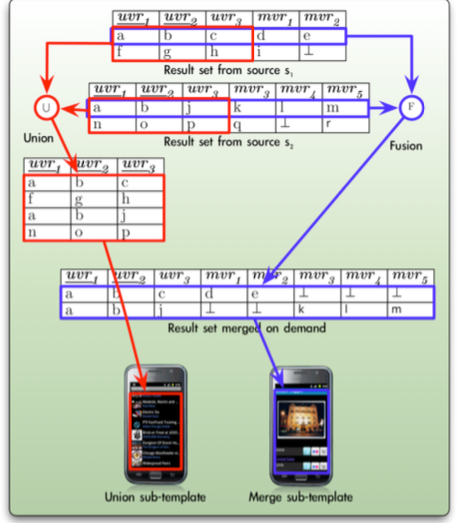
\includegraphics[width=0.5\textwidth]{2-nozioni-preliminari/Immagini/merge-union.png}
	\caption{Esempio di merge e union}\label{fig:merge-union}
\end{figure}

\section{Web Services\label{sec:web-services}}

Secondo la definizione formale fornita dal Consorzio W3C\footnote{Consorzio W3C: \url{https://www.w3.org/}} \virgolette{un Web Service è un sistema software creato allo scopo di permettere la comunicazione tra macchine attraverso una rete. \upe composto da un'interfaccia di programmazione, descritta in un linguaggio interpretabile dalle macchine (WSDL in particolare). [...]} \cite{world2004web}. In questa definizione viene citato l'utilizzo del protocollo SOAP: in realtà, qualche anno più tardi, la definizione è stata estesa \cite{w3c2004web}, includendo nell'elenco:

\begin{itemize}
	\item \emph{REST Web Services}, il cui obiettivo principale è la manipolazione di \emph{risorse} utilizzando operazioni che non necessitano di mantenere uno stato
	\item \emph{Servizi Web Arbitrari}, dove è possibile esporre a piacimento un insieme di operazioni
\end{itemize}

Il motivo principale che ha spinto verso questa scelta è da ricercare nella definizione stessa di \emph{web service}: l'obiettivo principale è quello di permettere lo scambio di informazioni tra macchine, favorendo l'interoperabilità tra sistemi e linguaggi di programmazione differenti. La maggior parte dei servizi utilizza il protocollo HTTP come livello di trasporto: questa scelta ha l'enorme vantaggio di poter sfruttare lo stesso protocollo già utilizzato per le comunicazioni via internet, così da ridurre i costi di gestione necessari per la messa in opera di un diverso protocollo. Nel corso del tempo sono nate diverse tipologie di servizi: alcuni, come SOAP, forniscono una struttura standardizzata da seguire per l'implementazione dei servizi compatibili mentre altri, come REST, forniscono delle linee guida sulla metodologia da seguire per l'implementazione del servizio, ma non sono dipendenti da nessuna tecnologia in particolare. La creazione di servizi che adempiono a uno specifico compito ha favorito un ulteriore aspetto: la composizione. \upe possibile creare dei servizi che ne sfruttano contemporaneamente diversi al fine di realizzare un processo più complesso \cite{weerawarana2005web}. Recentemente questo concetto è stato ulteriormente esteso con la realizzazione dei cosiddetti \emph{mashup} \cite{benslimane2008services}, applicazioni web che permettono di combinare assieme informazioni provenienti da diverse fonti dinamicamente, in modo da fornire un'esperienza utente migliore.

Di seguito vengono analizzate alcune tra le tecnologie e paradigmi più utilizzati per la creazione di servizi, tra cui SOAP, REST e GraphQL.

\subsection{SOAP\label{sec:soap-introduzione}}

\upe l'acronimo di \emph{Simple Object Access Protocol} e fornisce un framework per lo scambio di messaggi.  Utilizza come formato di risposta XML e nella maggior parte dei casi si appoggia al protocollo HTTP come livello di trasporto. Vengono scambiate delle \emph{buste}, che contengono le informazioni su come interrogare il servizio e come sono rappresentate le risposte. L'architettura SOAP viene distinta per tre caratteristiche principali:

\begin{enumerate}
	\item \textbf{Estensibilità}
	Le funzionalità di base possono essere ampliate attraverso l'u\-ti\-liz\-zo di estensioni
	\item \textbf{Neutralità}
	Non dipende da nessun protocollo di comunicazione in particolare. Quello più utilizzato è HTTP, ma esistono delle implementazioni per SMTP, TCP, UDP o JMS per citarne alcuni
	\item \textbf{Indipendenza}
	Può essere utilizzato da diversi linguaggi di programmazione
\end{enumerate}

In seguito, SOAP è stato utilizzato come base per altre tecnologie legate ai web services, come il \emph{Web Services Description Language} (WSDL), che è un'interfaccia di descrizione delle funzionalità fornite dal servizio, e l'\emph{Universal Description Discovery and Integration} (UDDI), che è un registro dove è possibile ricercare i servizi.

\subsection{REST\label{sec:rest-introduzione}}

\upe l'acronimo di \emph{REpresentational State Transfer} ed è uno stile architetturale che definisce determinati vincoli di comportamento per componenti, connettori e dati che compongono un sistema distribuito ipermediale. \emph{REST} è prima di tutto un paradigma: non vengono infatti menzionati nè i dettagli relativi all'implementazione dei componenti nè i protocolli da utilizzare proprio per concentrarsi sul ruolo dei componenti, sulle loro interazioni e come interpretare le informazioni. Il termine \emph{REpresentational State Transfer} è stato utilizzato per la prima volta nella tesi di dottorato di Roy Fielding \cite{fielding2000architectural}. \emph{REST} viene largamente utilizzato per descrivere i servizi web, in modo tale da non generare contraddizioni durante l'implementazione. I sistemi che rispettano i principi \emph{REST} vengono chiamati \emph{RESTful}. Nella maggior parte dei casi, i sistemi \emph{RESTful} comunicano attraverso i verbi standard del protocollo HTTP (GET, POST, PUT, DELETE, ecc.). Utilizza le \emph{web resources} come interfaccia per comunicare con i sistemi esterni, identificate tramite un \emph{Uniform Resource Identifier} (URI). L'applicazione delle linee guida definite dall'architettura permette di ottenere i seguenti vantaggi: performance, scalabilità, semplicità, manutenibilità, visibilità, portabilità e affidabilità.

I vincoli definiti dall'architettura sono:

\begin{itemize}
	\item \textbf{Client-server}
	C'è una separazione delle attività che devono essere eseguite sul client e sul server. Per esempio, i client non devono occuparsi della memorizzazione dei dati, che rimane interna al server, in modo da favorire la \emph{portabilità} del codice del client. Il server invece non deve preoccuparsi dell'interfaccia e dello stato dell'utente, in modo da rendere l'implementazione del server più semplice e \emph{scalabile}. Il client e il server possono essere sostituiti e sviluppati separatamente a patto che le interfacce tra di loro rimangono immutate
	\item \textbf{Stateless}
	Lo stato non deve essere assolutamente salvato sul server. Ogni richieste che proviene dal client deve contenere tutte le informazioni necessarie alla sua esecuzione. Sarà compito del client mantenere memorizzato lo stato corrente. Lo stato della sessione può però essere trasferito dal server verso un ulteriore servizio di memorizzazione, per esempio un database, per un periodo di tempo limitato. Al client viene affidato il compito di decidere quando è pronto a passare a un nuovo stato
	\item \textbf{Cacheable}
	Sia il client sia il server possono effettuare caching delle risposte. Le risposte devono innanzitutto definire se possono essere salvate in cache o meno, in modo da limitare le situazioni nelle quali il client utilizza informazioni non corrette o non più valide. Implementare un ottimo sistema di cache permette di ridurre il numero di interazioni tra il client e il server, migliorando la scalabilità e le performance del sistema
	\item \textbf{Layered system}
	Un client non può specificare se è connesso direttamente al server di più basso livello oppure a un server intermediario. L'utilizzo di server intermediari permette di migliorare la scalabilità del sistema, tramite load balancer e cache distribuite. Possono inoltre fornire ulteriori misure di sicurezza
	\item \textbf{Uniform interface}
	L'utilizzo delle \emph{uniform interface} permette di semplificare e disaccoppiare i vari componenti dell'architettura, rendendo possibile lo sviluppo indipendente delle varie parti del sistema. I quattro vincoli riguardo le \emph{uniform interface} sono:
	\begin{enumerate}
		\item \textbf{Identificazione delle risorse}
		Le singole risorse vengono identificate nella richiesta tramite, per esempio, un \emph{URI}. Le risorse sono concettualmente separate dalle rappresentazioni che vengono inviate al client. Per esempio, un server può inviare dati acquisiti dal database sotto forma di file HTML, XML o JSON, che sono diversi dalla rappresentazione interna del server
		\item \textbf{Manipolazione delle risorse tramite le rappresentazioni}
		Ogni rappresentazione di una risorsa che viene inviata al client deve contenere tutte le informazioni che permettano la modifica o l'eliminazione della risorsa
		\item \textbf{Messaggi autoesplicativi}
		Ogni messaggio deve contenere informazioni su come trattare l'informazioni che porta con sè, tramite per esempio i \emph{media type}
		\item \textbf{Sfruttamento dell'hypermedia (HATEOAS)}
		I client possono effettuare delle azioni che vengono dinamicamente messe a disposizione dal server tramite hypermedia (es.: link). A eccezione dello stato iniziale, il client conosce le attività che possono essere eseguite a partire da una data rappresentazione solamente tra quelle che espone
	\end{enumerate}
\end{itemize}

Applicando i principi REST alle API dei servizi web si ottengono quelle che vengono definite \emph{RESTful API}. Le \emph{RESTful API} che sfruttano il protocollo HTTP sono definite tramite le seguenti caratteristiche:

\begin{itemize}
	\item
	Possiedono un URI di base
	\item
	Definiscono un media type, che indica il formato della risposta, che nelle implementazioni più comuni è JSON
	\item
	Utilizzano i verbi standard del protocollo HTTP (es.: OPTIONS, GET, PUT, POST e DELETE)
	\item
	Mettono a disposizione dei link come referenza per passare alle risorse correlate
	\item
	Utilizzano dei link come referenza dello stato
\end{itemize}

Solitamente a una URI viene associata una funzione diversa in base al verbo con la quale viene chiamata, in modo da distinguere l'operazione che si vuole eseguire sull'elemento o collezione. Per esempio, eseguire una \virgolette{GET} su di un'elemento permette di recuperarne le informazioni mentre eseguire una \virgolette{PUT} crea un nuovo elemento.
%, come si può notare nell'esempio in Tabella \ref{table:esempio-rest-api}.

%\begin{table}[ht]
%	\caption{Esempio RESTful API}
%	\label{table:esempio-rest-api}
%	\noindent\makebox[\textwidth]{%
%	\begin{tabularx}{1.3\textwidth}{lXXXX}
%		\toprule
%		\thead{Risorsa} & \thead{GET} & \thead{PUT} & \thead{POST} & \thead{DELETE} \\
%		\midrule
%		\url{http://api.example.com/resources/} & \textbf{Elenca} le URI insieme a eventuali altri dettagli sulla collezione & \textbf{Sostituisce} la collezione con un'altra & \textbf{Aggiunge} un nuovo elemento alla collezione. L'URI viene generato automaticamente e restituito dall'operazione & \textbf{Elimina} l'intera collezione \\
%		\hline
%		\url{http://api.example.com/resources/item17} & \textbf{Restituisce} una rappresentazione dell'oggetto, espresso con un particolare \emph{media type} & \textbf{Sostituisce} l'elemento della collezione o, se non esiste, ne crea uno nuovo & \textbf{Crea} un nuovo elemento & \textbf{Rimuove} l'elemento dalla collezione \\
%		\bottomrule
%	\end{tabularx}}
%\end{table}

\section{Tecnologie utilizzate per il backend\label{sec:tecnologie-backend-background}}

In questa sezione si vuole fornire una panoramica sulle tecnologie che sono state utilizzate per lo sviluppo del backend. Verrà analizzato per prima il framework Node.js, con il quale è stata sviluppata la logica del backend. In seguito verranno descritti i due database utilizzati: MongoDB, per la persistenza dei dati, e Redis, per la gestione della cache.

\subsection{Node.js}

La logica del sistema è stata realizzata a partire da Node.js\footnote{Node.js: \url{https://nodejs.org/en/}}, un framework per lo sviluppo di applicazioni web basato sul linguaggio Javascript\footnote{Javascript Documentation: \url{https://developer.mozilla.org/en/docs/Web/JavaScript}}. Node.js è basato sul motore Javascript V8 di Google, realizzato con l'obiettivo principale di garantire ottime performance di esecuzione. Il framework permette la creazione di web server tramite l'ausilio di diversi \emph{moduli} che gestiscono le funzionalità di base, come il file system, le operazioni di rete, la crittografia, ecc. \upe compatibile con i sistemi operativi più diffusi e possono essere utilizzati tutti i linguaggi che una volta compilati producono codice Javascript, come CoffeScript o TypeScript. Per certi versi Node.js può essere considerato molto simile a PHP come ambito di utilizzo, la principale differenza è che le funzioni in Node.js non sono bloccanti, quindi è possibile eseguire attività in parallelo e utilizzare callback o promise per gestire il flusso di esecuzione, nel caso in cui le singole funzioni abbiano successo o meno. Questa scelta di utilizzare un'architettura di tipo \emph{event-driven} permette la realizzazione di web server estremamente scalabili senza utilizzare più thread. Node.js infatti lavora solo su un singolo core, tranne ne caso in cui vengano avviate più istanze separate. Il parallelismo gestito tramite eventi permette di simulare un sistema multithread, riducendo però in maniera significativa la complessità di sviluppo.

\subsection{MongoDB}

Come database è stato scelto di utilizzare MongoDB\footnote{MongoDB: \url{https://www.mongodb.org/}}. MongoDB fa parte della categoria NoSQL, in quanto abbandona lo schema relazionale classico basato su tabelle in favore di uno basato sui documenti. Ogni documento ha una struttura simile a un file JSON, che in MongoDB viene nominato BSON. A differenza dei database relazionali che hanno uno schema ben definito a priori, in MongoDB viene preferito uno schema dinamico, cioè che varia in base alle esigenze dello sviluppatore. Questa caratteristica permette di sviluppare in maniera più semplice e rapida le applicazioni e di integrare facilmente determinate tipologie di dato. La struttura a documento prevede però un approccio differente nella fase di modellazione, in quanto applicare uno schema adatto a un sistema relazionale in MongoDB porterebbe a diverse inefficienze. Per esempio, chi è abituato a un database relazionale deve essere consapevole che in MongoDB non esiste l'operatore di JOIN, bensì viene fornita la possibilità di salvare dei sotto-documenti all'interno di un documento. Per esempio, se si vuole memorizzare un libro che ha più autori è possibile salvare l'elenco degli autori, insieme a eventuali altri suoi dati, all'interno del documento contenente le informazioni del libro\footnote{Questo è solo un esempio indicativo, non è una soluzione ottima in quanto un autore può pubblicare più di un libro e utilizzando questo schema si otterrebbe duplicazione delle informazioni.}. Un'altra caratteristica di MongoDB è la flessibilità nella composizione delle query: possono essere specificate sui campi, su un range di valori o tramite un'espressione regolare. Sono sempre ammesse proiezioni degli attributi che si vogliono visualizzare nei risultati. Sempre per interrogare i dati si possono utilizzare funzioni \emph{MapReduce} e di \emph{aggregazione}. In particolare quest'ultima permette di ottenere un risultato simile all'operatore GROUP BY dei database SQL, ma fornisce inoltre la flessibilità di concatenare più operazioni per formare una \emph{pipeline}. Mette a disposizione anche il comando \emph{\$lookup} per effettuare un'unione tra documenti diversi, al fine di simulare un'operazione di JOIN. MongoDB permette di definire degli \emph{indici} sui campi che vengono utilizzati di frequente nelle query per velocizzarne l'esecuzione. Una caratteristica che rende MongoDB estremamente scalabile è la possibilità di eseguire multiple istanze su macchine diverse, permettendo al sistema di scalare orizzontalmente. Sarà compito di MongoDB gestire le chiamate e selezionare il nodo dove effettuare la richiesta, tramite un sistema di load-balancing. Questa caratteristica viene agevolata dalla struttura del file system utilizzato da MongoDB, chiamato \emph{Grid File System}, che gestisce la divisione dei documenti in diversi \virgolette{pezzi}. Oltre al load-balancing, che viene utilizzato per migliorare le prestazioni, è possibile anche utilizzare altre macchine come \emph{repliche}, in modo da garantire la sicurezza dei dati nel caso di guasti.

Il fatto che MongoDB memorizzi i file in un formato dalla struttura molto simile a un JSON agevola l'integrazione con Node.js, che a sua volta utilizza oggetti semplicemente convertibili in formato JSON.

\subsection{Redis}

Oltre a un database che garantisse la persistenza dei dati più importanti, si è resa necessaria l'adozione di un altro database per effettuare  caching delle risposte ricevute dai servizi e per memorizzare informazioni relative alle sessioni degli utenti. La scelta in questo caso è ricaduta su Redis\footnote{Redis: \url{http://redis.io/}}. Redis fornisce un database interamente memorizzato in memoria, quindi estremamente rapido nell'evadere le richieste, basato su di una struttura di tipo \emph{chiave-valore}. Queste caratteristiche, insieme al fatto che quanto viene salvato un dato è possibile impostare un intervallo di tempo scaduto il quale l'elemento viene eliminato, lo hanno reso il candidato perfetto per svolgere questo compito.

\subsection{GraphQL\label{sec:graphql-introduzione}}

\emph{GraphQL}\footnote{GraphQL: \url{http://graphql.org/}} è, come suggeriscono le ultime due lettere del nome, un \emph{query language}, creato come supporto alla realizzazione di applicazioni client, che mette a disposizione una sintassi intuitiva e flessibile e un sistema che permette al client di specificare i requisiti e le interazioni sui dati \cite{website:graphql-specs}. Rispetto all'approccio REST, \emph{GraphQL} permette di effettuare richieste più efficienti dei dati ed evita la duplicazione della logica lato server che può verificarsi nel caso di endpoint personalizzati. Una delle principali differenze rispetto a REST riguarda la possibilità di lasciare al client la scelta dei dati da ricevere. Questa modifica nasce dall'idea che è il client a conoscere nel dettaglio quali dati servono per comporre la view e quindi gli viene delegata la responsabilità di richiedere solo quelli essenziali all'interno della query.

Alla base di \emph{GraphQL} ci sono i seguenti principi:

\begin{itemize}
	\item \textbf{Gerarchico}
	Una buona parte dei prodotti sviluppati implica la creazione e manipolazione di view gerarchiche. Per mantenere coerenza con la struttura delle applicazioni, le query \emph{GraphQL} sono esse stesse strutturate gerarchicamente. La query viene plasmata esattamente come i dati che deve restituire. \upe un metodo naturale per permettere ai client di descrivere i vincoli sui dati
	\item \textbf{Basato sul prodotto}
	\emph{GraphQL} è stato creato tenendo ben presenti i requisiti delle view e del come gli sviluppatori di front-end li esplicitano
	\item \textbf{Tipizzato}
	Ogni server \emph{GraphQL} definisce il proprio schema specifico per l'applicazione in uso. Le query vengono eseguite a partire dal contesto definito da questo schema. Inoltre vengono effettuati dei controlli al fine di verificare che la query sia sintatticamente corretta e valida  prima di essere eseguita
	\item \textbf{Query definite dal client}
	Negli schemi viene inoltre definito il formato della risposta, compresa la tipologia di ogni dato. Sarà poi il client a specificare esattamente quali sono le informazioni che gli interessano. Rispetto ad altri approcci, dove è il server a decidere quali dati restituire ai client, in \emph{GraphQL} invece vengono restituiti solamente i dati che vengono richiesti e nulla di più
	\item \textbf{Introspettivo}
	Qualsiasi schema \emph{GraphQL} può essere interrogato tramite query. In questo modo è possibile conoscere la struttura globale dello schema, così come le query che sono permesse e quali dati possono essere richiesti. Queste introspezioni vengono utilizzate da vari tool per avere una visione completa dello schema che viene esposto dal server
\end{itemize}

\begin{figure}[ht]
	\begin{minipage}[t]{0.49\textwidth}
		\begin{listing}[H]
			\inputminted{text}{2-nozioni-preliminari/Codice/esempio_query_graphql.graphql}
			\caption{Esempio query GraphQL}
			\label{lst:esempio-query-graphql}
		\end{listing}
	\end{minipage}%
	\hspace{2mm}%
	\begin{minipage}[t]{0.49\textwidth}
		\begin{listing}[H]
			\inputminted{json}{2-nozioni-preliminari/Codice/esempio_risposta_graphql.json}
			\caption{Esempio di risposta}
			\label{lst:esempio-risposta-graphql}
		\end{listing}
	\end{minipage}	
\end{figure}

Nel Listato \ref{lst:esempio-query-graphql} viene riportato un semplice esempio di query scritta tramite \emph{GraphQL}. Con questa query si vogliono acquisire i dati relativi all'utente con identificativo 2, e in particolare si è interessati a ricevere il suo \emph{nome} e \emph{cognome}. Nel Listato \ref{lst:esempio-risposta-graphql} viene invece mostrato un esempio di risposta che viene ricevuta dalla server.

\emph{GraphQL} fornisce inoltre un'altra funzionalità estremamente utile: le \emph{connessioni}. Una \emph{connessione} permette a un oggetto di definire i legami che ha con altri oggetti, anche di tipo diverso dal proprio. In questo modo è possibile richiedere direttamente le informazioni riguardo altri oggetti tramite un'unica query; questa caratteristica non è presente nei sistemi REST e permette di ottenere un netto miglioramento delle performance. Infatti nei sistemi REST, per richiedere le rappresentazioni correlate sono necessarie \emph{n} query, dove \emph{n} è il numero di risorse da richiedere. Con GraphQL invece è sufficiente una sola richiesta, nella quale viene specificato che si è interessati anche alle altre risorse. Inoltre, GraphQL mette a disposizione per ogni connessione la \emph{paginazione} dei risultati, ossia la possibilità di richiedere un determinato numero di elementi a ogni richiesta. A ogni oggetto viene automaticamente associato un \emph{token} che lo identifica univocamente: in questo modo è possibile chiedere ulteriori elementi in una seconda query, specificando il \emph{token} dell'oggetto dal quale si desidera partire.

\begin{figure}[ht]
	\hspace*{-1.2cm}
	\begin{minipage}[t]{0.55\textwidth}
		\begin{listing}[H]
			\inputminted{text}{2-nozioni-preliminari/Codice/esempio_connessione_graphql.graphql}
			\caption{Esempio connessione GraphQL}
			\label{lst:esempio-connessione-graphql}
		\end{listing}
	\end{minipage}%
	\hspace{2mm}%
	\begin{minipage}[t]{0.55\textwidth}
		\begin{listing}[H]
			\inputminted{json}{2-nozioni-preliminari/Codice/esempio_risposta_connessione_graphql.json}
			\caption{Esempio di risposta}
			\label{lst:esempio-risposta-connessione-graphql}
		\end{listing}
	\end{minipage}	
\end{figure}

Nel Listato \ref{lst:esempio-connessione-graphql} viene mostrata una query più complessa della precedente. La \emph{connessione} viene definita da \virgolette{friendConnection}, che viene utilizzata per recuperare gli amici dell'utente corrente. Si vuole far notare che gli oggetti che vengono restituiti nel campo \virgolette{friends} sono dello stesso tipo dell'utente richiesto in origine: questo vuol dire che è possibile produrre infiniti livelli gerarchici. Se, all'interno di un utente amico, si specifica di nuovo la connessione \virgolette{friendConnection}, verranno restituiti anche gli amici di quello specifico utente. Altro punto interessante, come citato in precedenza, delle \emph{connessioni} riguarda la possibilità di richiedere solo un sottoinsieme dei risultati: nell'esempio vengono richiesti solamente i primi due amici dell'utente. Come si può notare nel Listato \ref{lst:esempio-risposta-connessione-graphql}, vengono restituiti solamente i primi due amici, nonostante il campo \virgolette{totalCount} indichi che l'utente ha in totale 13 amici. Tramite ulteriori query possono essere richiesti gli altri amici dell'utente.

\section{Panoramica su cross platform mobile e tecnologie utilizzate}\label{sec:panoramica-cross-platform-mobile}

Al momento di scegliere come implementare l'applicazione mobile per CAMUS sono state considerate due opzioni: la creazione di un'applicazione nativa inizialmente solo per Android, per poi estendere la compatibilità su iOS, oppure l'utilizzo di strumenti cross platform, funzionanti su più di un sistema operativo mobile.
Questa esigenza è nata dal fatto che il mercato delle app mobile sta crescendo in maniera esponenziale e le competenze richieste agli sviluppatori sono molto variegate per sviluppare applicazioni native.
Per esempio per quanto riguarda lo sviluppo iOS è necessario conoscere come linguaggi di programmazioni Objective-C e Swift, per Android ci si basa principalmente su Java e per Windows Phone è necessario utilizzare C\#, senza dimenticare altri sistemi operativi meno diffusi o emergenti (Tizen, Ubuntu Touch, ecc.). La tipologia di strumenti che permettono di sviluppare un'applicazione scrivendo una sola volta il codice ed eseguirla su diversi sistemi operativi mobili è detta \emph{cross-platform}
Gli strumenti di sviluppo \emph{cross-platform} solitamente si basano sul principio di \virgolette{write once run everywhere}, cioè il codice viene scritto una volta sola per creare applicazioni per diverse piattaforme, permettendo quindi di limitare le competenze richieste ai programmatori. 
\upe possibile identificare due famiglie di strumenti per la programmazione multi piattaforma:

\begin{enumerate}
	\item \textbf{Rendering tramite componenti nativi}
	In questa famiglia il rendering dell'applicazione viene fatto utilizzando le API grafiche native del sistema operativo di destinazione.
	Al fine di ottenere ciò è necessario implementare una traduzione in codice nativo a partire dal linguaggio utilizzato per programmare. Ad esempio in Xamarin si programma utilizzando C\# per programmare sia in Android che in iOS ed è possibile effettuare \emph{Linking} con le librerie di sistema dei due sistemi operativi e fornire una migliore esperienza d'uso per l'utente. Anche per quanto riguarda altri strumenti come React Native o Native Script\footnote{Native Script: \url{https://www.nativescript.org/}} che utilizzano JavaScript viene riproposto lo stesso principio compositivo
	\item \textbf{Rendering tramite WebView}
	In questo caso la costruzione della maggior parte dell'applicazione è svolta utilizzando una \emph{Web View}, cioè viene mostrata una pagina web all'interno di un contenitore nativo.
	In questo caso è possibile programmare l'applicazione come se fosse una pagina web, implementandolo allo stesso modo di un sito web per browser. Nonostante si tratti di un'implementazione non molto legata alla logica nativa, è possibile in alcuni casi permettere un'interazione dell'applicazione con i sensori del dispositivo.
	Questo modello offre un'infinità di possibilità implementative a livello grafico e una elevata capacità di adattamento a diversi dispositivi, tuttavia le prestazioni possono risentire del fatto che si stia interagendo con una pagina web e non con una applicazione nativa
\end{enumerate}

Per la creazione di CAMUS si è scelto di utilizzare anche lato \emph{frontend} degli strumenti che siano implementabili in maniera semplice e dove la suddivisione in moduli singoli riutilizzabili assuma un ruolo di primo piano. Per questo motivo si è scelto di utilizzare degli strumenti tecnologici che sono all'avanguardia nello svolgere questo compito, come React e la sua derivazione per la programmazione mobile React Native. Successivamente è introdotta la parte logica dell'applicazione con il funzionamento architetturale dell'aggiornamento dati, con il paradigma Flux.

\subsection{React}\label{sec:react}

React\footnote{React:\url{https://facebook.github.io/react/}} nasce come libreria open-source rilasciata nel 2013 da Facebook, che permette di ottimizzare le visualizzazioni delle pagine HTML, utilizzando componentine racchiudono altri specificati come HTML tag personalizzati.
Essa proviene da XHP\footnote{XHP: \url{http://facebook.github.io/xhp-lib/}}, che è un framework HTML per il linguaggio PHP creato sempre in Facebook per gestire tutta la logica del social network. L'impiego di \emph{React} è stato inizialmente nel newsfeed di \emph Facebook nel 2011 e più tardi nel sito web di Instagram.
Le principali funzionalità in React sono le seguenti:

\begin{itemize}
	\item \textbf{Virtual DOM}
	React crea una propria struttura dati in memoria, che calcola le differenze risultanti e aggiorna il DOM HTML risultante nella pagina in modo efficiente. In questo modo il programmatore può scrivere codice come se l'intera pagina è ricaricata ogni volta, mentre il motore React a stabilire quali siano i componenti che è necessario sostituire e quali no
	\item \textbf{JSX}
	I componenti React utilizzano JSX\footnote{JSX: \url{https://jsx.github.io/}}, un linguaggio basato su JavaScript che introduce la tipizzazione delle variabili e un sistema di classi ben definito come in Java. Inoltre porta ottimizzazioni a livello di compilazione permettendo all'applicazione di essere più performante rispetto a normale codice JavaScript. \upe comunque possibile scrivere la propria applicazione utilizzando JavaScript, con un metodo che permette la conversione in codice JSX
	\item \textbf{One-way data flow}
	Le proprietà, un set di valori immutabili, sono passati al componente figlio all'interno del suo tag HTML.Il componente figlio non può modificare direttamente nessuna proprietà che gli è stata passata, ma può passare funzioni che possono modificare il valore. 
	L'unidirezionalità del flusso dati viene specificata nell'architettura Flow, che verrà spiegata nella Sezione \ref{sec:flux}
\end{itemize}

\subsection{React Native}\label{sec:react-native}

React Native\footnote{React Native: \url{https://facebook.github.io/react-native/}} è una libreria open-source rilasciata nel 2015 sempre da Facebook, proponendosi come implementazione del framework React per quanto riguarda le applicazioni mobile.
Le principali differenze con React sono dovute alla difficoltà maggiore di sviluppare un framework per le applicazioni mobile. 
Quando si sviluppa sul web, semplicemente si salvano i file modificati e si ricarica la pagina, cosa che non è possibile fare con le applicazioni mobile, perché è necessaria una nuova compilazione per vedere i cambiamenti apportati.
Per risolvere questo problema, in React Native ci si basa sull'utilizzo di un server locale in \emph{node.js} che permette il caricamento delle modifiche dell'applicazione sul dispositivo senza ricompilare l'applicazione (Figura \ref{fig:flusso-sviluppo-react-native}) Questo server, il quale ha la funzione di packager, invia un bundle contente tutti i file JavaScript necessari per far funzionare l'applicazione. Questo funziona fino a quando le modifiche sono relative esclusivamente alla parte di codice JavaScript, mentre per quanto riguarda le modifiche a livello di codice nativo è sempre necessaria una nuova compilazione. Per esempio, quando è stato il momento di installare alcune librerie grafiche collegate ad elementi nativi è stato necessario apportare modifiche anche ai file di configurazione dei progetti Android e iOS, dato che diventavano necessari anche file aggiuntivi alla compilazione.

\begin{figure}[ht]
	\centering
	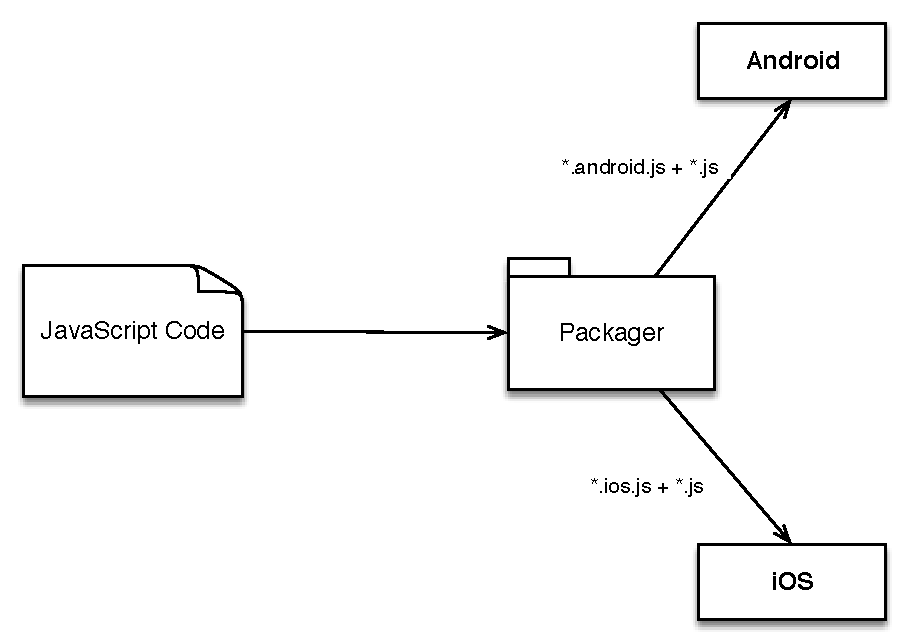
\includegraphics[width=0.8\textwidth]{6-implementazione-app/immagini/flusso-sviluppo-react-native.pdf}
	\caption{Flusso di sviluppo React Native\label{fig:flusso-sviluppo-react-native}}
\end{figure}

Con React Native è possibile migliorare l'esperienza d'uso sulle piattaforme mobile rispetto al web. Come primo aspetto si può accedere ai componenti specifici dell'interfaccia utente, come le mappe, i picker e gli switch, anche se tuttavia possono essere modificati nella loro implementazione.

\subsection{Flux}\label{sec:flux}

Flux\footnote{Flux: \url{https://facebook.github.io/flux/}} è un pattern architetturale creato da Facebook per gestire il flusso dei dati all'interno dell'applicazione. \upe complementare alla gestione delle view di React, in cui i componenti sfruttano un flusso di dati unidirezionale, come espresso in Figura \ref{fig:flux}.

\begin{figure}[ht]
	\centering
	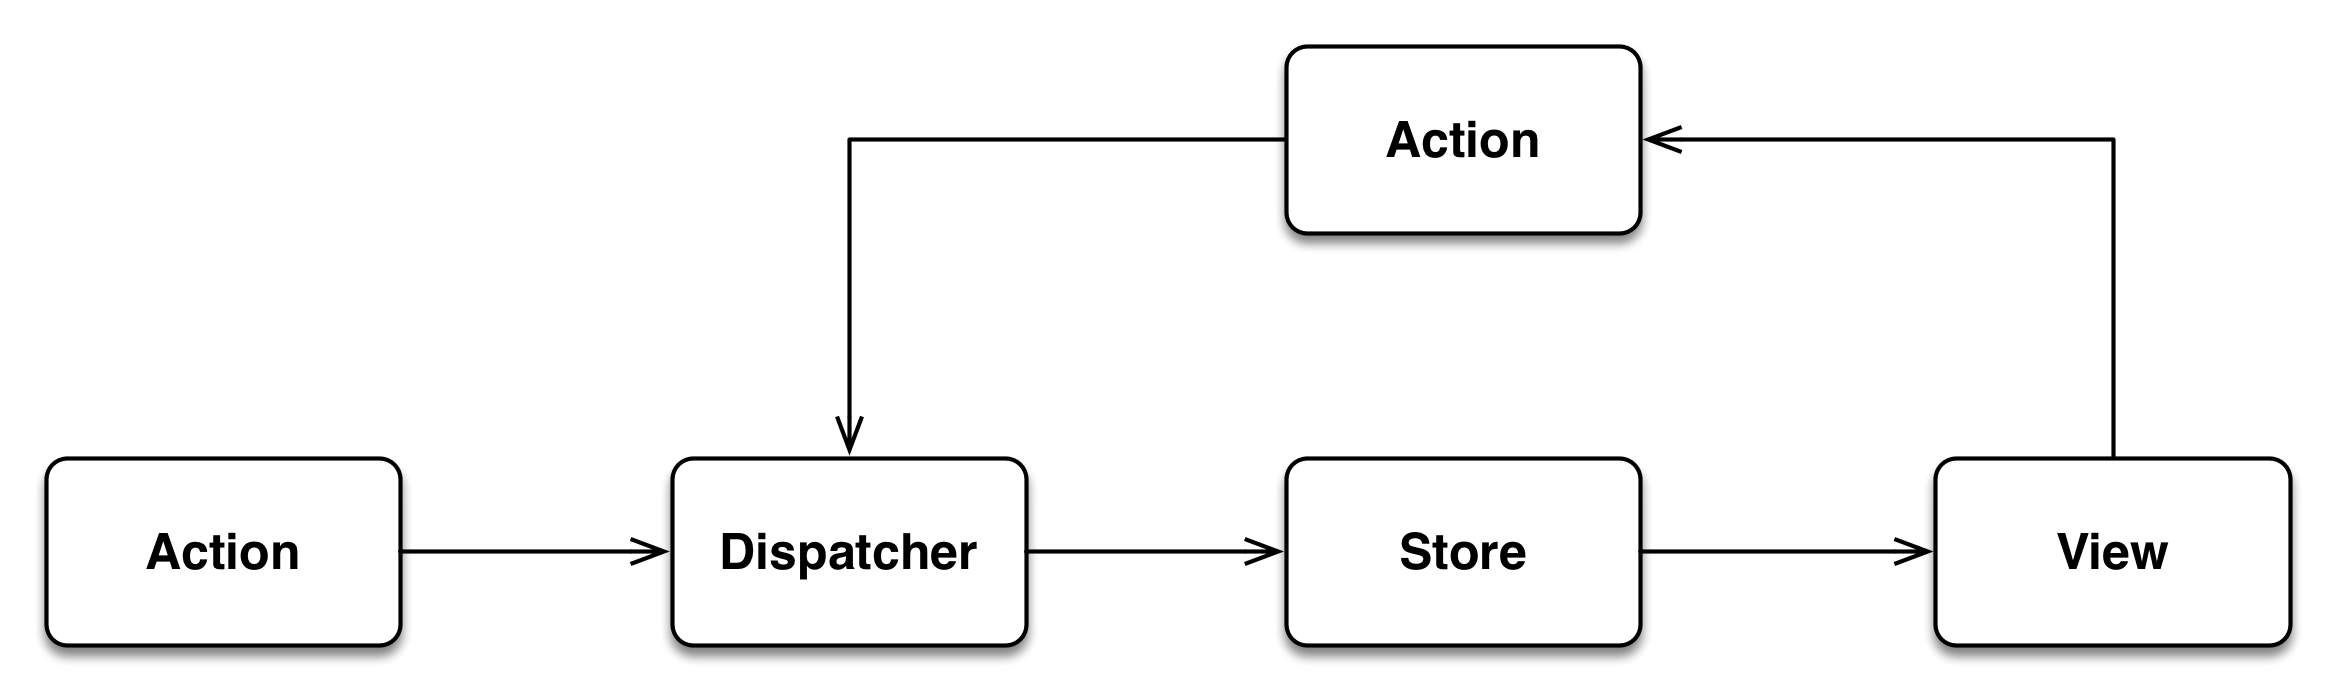
\includegraphics[width=\textwidth]{6-implementazione-app/immagini/flux.png}
	\caption{Flusso dati unidirezionale Flux}\label{fig:flux}
\end{figure}

Si tratta fondamentalmente di una modifica del pattern MVC (Model View Controller), al quale vengono effettuate alcune modifiche.
Le applicazioni Flux, come si vede nella medesima figura, hanno quattro tipologie di componenti principali:

\begin{enumerate}
	\item \textbf{Dispatcher}
	Il \emph{Dispatcher} è l'hub centrale che controlla tutto il flusso dei dati dell'applicazione. \upe essenzialmente un registro di callback alle \emph{Store} e possiede un meccanismo semplice per distribuire le \emph{Action} verso le \emph{Store}. Man mano che l'applicazione cresce di dimensioni, il \emph{Dispatcher} assume un'importanza sempre maggiore, perché può essere sfruttato per gestire le dipendenze tra le \emph{Store} invocando le callback registrate in un ordine specifico, talvolta anche attendendo la conclusione dell'aggiornamento delle altre \emph{Store} 
	\item \textbf{Store}
	Le \emph{Store} contengono lo stato dell'applicazione e la logica, e il loro ruolo è molto simile al modello nel pattern MVC, ma in Flux hanno il compito di modellare lo stato per un particolare dominio all'interno dell'applicazione
	\item \textbf{View}
	L'implementazione delle view proposta da React si sposa perfettamente con quella necessaria per Flux. Si tratta di un misto tra la view e il controller in MVC, perché permette al codice di ricevere i dati dalle store e passare questi dati direttamente ai discendenti per creare ogni singola sezione della pagina. Quando riceve un evento dalle \emph{store}, richiede i nuovi dati attraverso i \emph{getter} delle \emph{store}, per poi aggiornare il proprio stato interno e renderizzarlo a cascata utilizzando tutti i sottocomponenti.
	\item \textbf{Action}
	Con il termine \emph{Action} si intende il payload di dati che viene mandato al metodo esposto dal \emph{dispatcher}, il quale come espresso nella sua spiegazione, poi si occupa di inviare i dati alle \emph{store}.
\end{enumerate} 

Nell'applicazione è stato scelto di utilizzare la libreria \emph{Alt.js}\footnote{Alt.JS: \url{http://alt.js.org/}} una libreria diversa da quella originale di Flux creata da Facebook, che, pur mantenendo un'ar\-chi\-tet\-tu\-ra funzionale simile, presenta alcune semplificazioni:

\begin{itemize}
	\item
	Non è necessario implementare il \emph{Dispatcher}, componente che è già fornito dalla libreria. È necessario fornire soltanto le \emph{Actions}  e le \emph{Stores}
	\item
	Le actions sono molto simili a quelle definite da Flux. Nel metodo che le definisce il dato ritornato alla fine viene automaticamente inviato al \emph{Dispatcher} di Alt
	\item
	Nelle \emph{Store} è necessario mappare l'operazione che controlla il corretto aggiornamento dei dati con le \emph{Actions} corrispondenti
	\item
	Il posizionamento delle operazioni preliminari al salvataggio dei dati è indifferente se sia nelle \emph{Actions} o nelle \emph{Stores} e può essere svolto prima o dopo l'operazione di dispatch di Alt, perché come spiegato nel punto precedente \emph{Actions} e \emph{Stores}
\end{itemize}

\section{Stato dell'arte\label{sec:stato-arte}}

In questa sezione vengono presentati alcuni strumenti già esistenti per quanto riguarda l'utilizzo dei mashup, quindi con l'integrazione e la fruizione dei servizi, e alcuni esempi di applicazioni che si adattano al contesto dell'utente.

\subsection*{Swagger}

Swagger \footnote{Swagger: \url{http://swagger.io}} è uno dei servizi più famosi per la definizione di interfacce REST per i servizi.
Lo scopo di Swagger è di definire un'interfaccia standard e indipendente dal linguaggio utilizzato per le diverse API al fine di permettere la scoperta e la comprensione delle risorse di un servizio, senza accedere ai suoi parametri tecnici (es.: codice sorgente, documentazione o ispezione del traffico di rete). Una volta definiti i servizi via Swagger, un consumatore può interagire con il servizio remoto implementando una minima parte di logica.
Swagger è quindi, tecnicamente parlando, una specifica formale supportata da un grande ecosistema di strumenti aggiuntivi, che comprende interfacce utente frontend, librerie di codice a basso livello e soluzioni commerciali per gestire le API.
Per poter descrivere la propria API con Swagger ci sono diversi approcci disponibili:

\begin{itemize}
	\item \textbf{Top-down}
	L'approccio top-down considera per prima la definizione del servizio che si vuole avere come output e successivamente genera l'applicazione. Per la prima operazione lo strumento fornito è lo \emph{Swagger Editor} (Figura \ref{fig:swagger}), che permette la definizione del nuovo servizio, mentre per la seconda operazione lo strumento utilizzato è \emph{Swagger Codegen}
	\item \textbf{Bottom-up}
	Nel caso in cui si ha una già API REST esistente e si vuole creare una nuova definizione si usa un approccio bottom-up. \upe possibile creare la definizione manualmente utilizzando lo \emph{Swagger Editor} oppure, nel caso si utilizzi uno dei framework supportati (es.: JAX-RS, Node.js, ecc.), è possibile generare in modo automatico la definizione Swagger
\end{itemize}

\begin{figure}[ht]
	\centering
	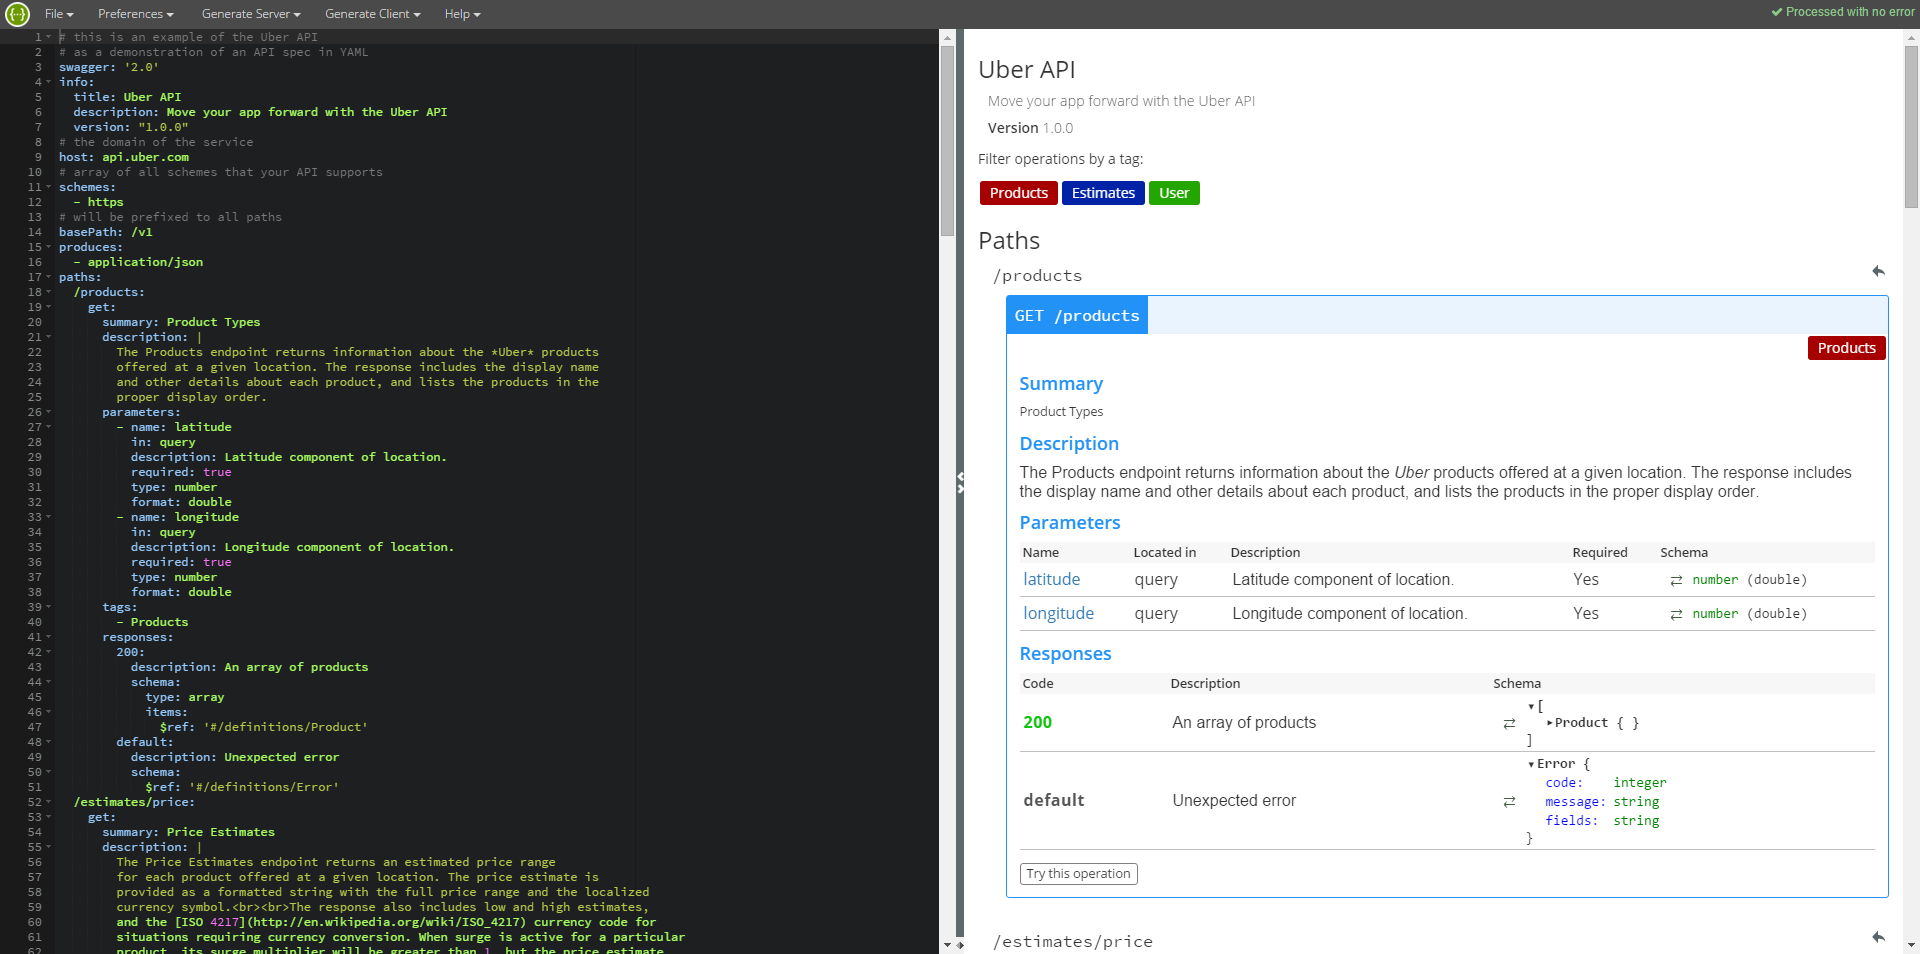
\includegraphics[width=\textwidth]{2-nozioni-preliminari/Immagini/swagger.png}
	\caption{Esempio Swagger Editor}\label{fig:swagger}
\end{figure}

Nel caso in cui si utilizzi una API e se ne voglia integrare un'altra che già possiede una definizione Swagger, si può utilizzare la versione online della \emph{Swagger UI} per esplorarla e successivamente lo \emph{Swagger Codegen} per generare la libreria client desiderata.

\begin{figure}[ht]
	\centering
	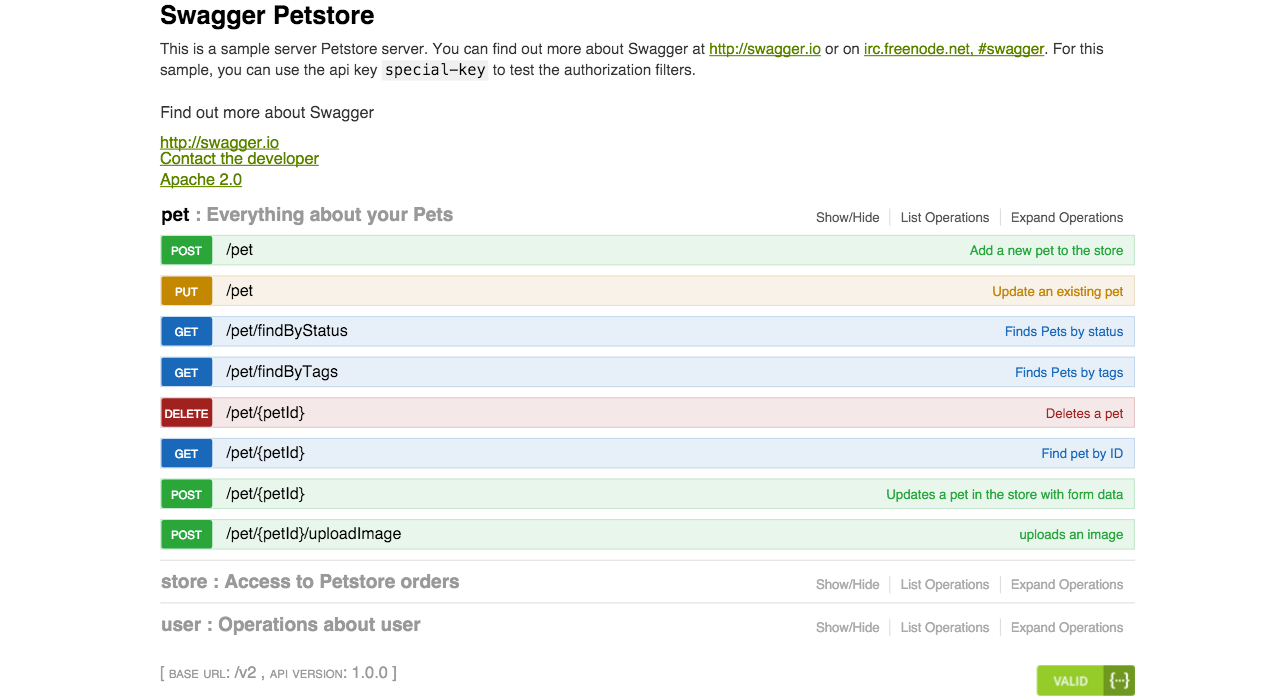
\includegraphics[width=\textwidth]{2-nozioni-preliminari/Immagini/swagger-petstore.png}
	\caption{Esempio API risultante Swagger}\label{fig:swagger-petstore}
\end{figure}

Nell'esempio in Figura \ref{fig:swagger-petstore} è presente una descrizione del servizio che è possibile generare con Swagger. In questo caso si tratta di un interfaccia di tipo REST con le operazioni CRUD, spiegate nel dettaglio in \ref{sec:web-services} e gli endpoint che è possibile invocare.

\subsection*{Appery.io}

Appery.io è uno strumento basato sul cloud che offre la possibilità di velocizzare lo sviluppo di applicazioni mobile e responsive. Ha due funzionalità principali: la costruzione di applicazioni mobile in maniera rapida e l'offerta di un servizio di Mobile Backend as a service (MBaaS).
Con il servizio di App Builder, è possibile creare applicazioni per dispositivi mobili che possono girare sui sistemi operativi più diffusi come iOS, Android e Windows Phone, a partire da un unica implementazione logica.
\upe possibile creare applicazioni di due tipi:

\begin{enumerate}
	\item \textbf{Hybrid Apps}
	Creare applicazioni ibride che utilizzano API comuni e indipendenti dal sistema operativo, che girano in modo coerente su iOS, Android e Windows Phone, integrando il supporto per i framework più diffusi come Apache Cordova (precedentemente conosciuto come PhoneGap), Ionic e jQuery Mobile. In questo modo è possibile fornire all'applicazione le potenzialità delle applicazioni completamente native, senza la necessità di imparare diversi linguaggi nativi. Si possono sfruttare inoltre tutti i plug-in disponibili per i vari framework, per implementare funzionalità più avanzate rispetto a quelle fornite dal framework stesso
	\item \textbf{Responsive Web Apps}
	Con il supporto a Bootstrap, il framework UI per le interfacce di tipo responsive, è possibile creare applicazioni web che adattano la modalità con la quale vengono visualizzate in base al tipo di dispositivo e alla dimensione dello schermo
\end{enumerate}

Per poter creare le applicazioni si utilizzano paradigmi di \emph{Visual Development} in modo da permettere la creazione rapida e intuitiva di nuove applicazioni, semplicemente usando \emph{drag \& drop}. \upe possibile sfruttare diversi template messi a disposizione da Appery.io per avere una base di partenza per alcune applicazioni comuni. Altrimenti, se si vuole ottenere maggiore flessibilità si può creare uno schema da zero. Viene anche fornita la possibilità di acquisire dati da servizi esterni, che possono essere associati utilizzando l'editor di Visual Data Mapping, anche scrivendo frammenti di codice personalizzati per garantire la massima adattabilità alle esigenze dell'utente. Le principali fasi che coinvolgono la realizzazione di un'applicazione sono:

\begin{figure}[ht]
	\centering
	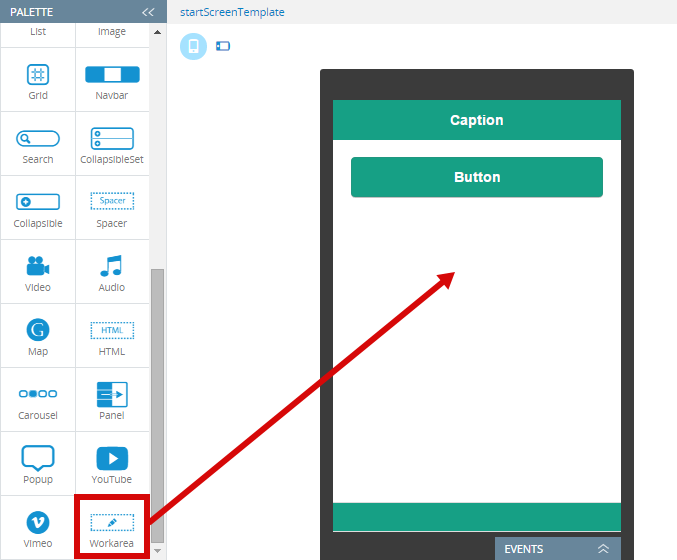
\includegraphics[width=\textwidth]{2-nozioni-preliminari/Immagini/appery-visual-composition.png}
	\caption{Composizione visuale in Appery.io}\label{fig:appery-visual-composition}
\end{figure}

\begin{itemize}
	\item \textbf{Development}
	La costruzione delle applicazioni è svolta in modo modulare, con componenti riutilizzabili in maniera veloce e semplice, come in Figura \ref{fig:appery-visual-composition}. Possono essere già presenti oppure creati ex-novo. Il tipo di struttura dati utilizzato, invece, è di tipo \emph{model-based}, in particolare è usato il pattern MVC (Model View Controller). Anche per quanto riguarda lo storage dei dati la soluzione scelta per l'interazione dell'utente è di tipo visuale, tramite la \emph{Storage API}, che permette di gestire le variabili in modo semplice
	\item \textbf{Deployment}
	Successivamente alla fase di sviluppo, in Appery.io è presente anche una parte per poter esportare la propria applicazione per le diverse piattaforme. In particolare, il metodo più veloce per poter diffondere l'app appena creata è l'utilizzo di un QR code. \upe sufficiente inviare questo codice per permettere di scaricare l'applicazione sul dispositivo. Oltre a questo metodo è possibile esportare l'applicazione come sorgenti HTML5/CSS oppure come progetti per gli IDE di sviluppo native come Android Studio, XCode o Visual Studio
	\item \textbf{Testing}
	\upe considerato anche l'aspetto del testing, sia per quanto riguarda HTML5 sia per  le app native.
	Nel primo caso è possibile eseguire testing istantaneamente nel browser o direttamente sul telefono, mentre nel secondo caso è supportato anche l'offline testing, cioè è possibile fare test di unità e di integrazione senza installare l'app sul dispositivo
	\item \textbf{Administration}
	La parte amministrativa è la parte che si riferisce al Mobile Backend as a Service (MBaaS) e permette di gestire tutta la parte di logica e storage sul cloud. Per quanto riguarda questo aspetto è presente in Appery.io una console di controllo, con la quale è possibile inviare notifiche push, controllare i certificati e le API key necessarie all'app, condividere lo sviluppo con altri utenti, gestire i ruoli del team di sviluppo e controllare i rilasci delle versioni dell'applicazione
\end{itemize}

\subsection*{Karma}

Karma\footnote{Karma: \url{http://usc-isi-i2.github.io/karma/}} è uno strumento di integrazione dati sviluppato dalla University of Southern California, che permette agli utenti di creare rapidamente e facilmente una nuova rappresentazione dei dati  da diverse fonti, come database, web API e documenti di diversa natura (XML, JSON, KML, ecc.). Gli utenti possono integrare le informazioni modellandole tramite un'ontologia di loro scelta. Questa attività viene svolta interamente tramite un'interfaccia grafica, in modo da semplificare il processo. 
Dopo questa operazione è possibile interagire con il sistema per correggere il modello generato in modo automatico ed è possibile trasformare i dati per normalizzarli. Una volta che il modello è completo, gli utenti possono pubblicare i nuovi dati come RDF o salvarli su un database.
Oltre a queste funzionalità, altre caratteristiche di Karma sono le seguenti:

\begin{itemize}
	\item \textbf{Ease of use}
	L'utente, utilizzando tecniche di programmazione per esempi e algoritmi  di ottimizzazione (es.: Steiner tree), perfeziona il modello generato in modo automatico utilizzando un interfaccia grafica che maschera la complessità delle regole di mapping usate
	\item \textbf{Semantic Models}
	Karma permette agli utenti di combinare diverse ontologie per permettere loro di mappare i loro dati a vocabolari standard
	\item \textbf{Scalable Processing}
	Anche la scalabilità è un elemento importante in Karma; infatti gli utenti lavorano con un sottoinsieme dei loro dati, permettendo di creare un'interfaccia utente dove essi definiscono il modello di integrazione dei dati. Dopo questo passaggio, il sistema usa questi modelli in modalità batch per integrare una quantità maggiore di dati
	\item \textbf{Data Transformation}
	Viene offerta un'interfaccia di programmazione per esempi che permette all'utente di definire le operazioni di trasformazione dei dati per poter restituire un unico formato comune
\end{itemize}

\begin{figure}[ht]
	\centering
	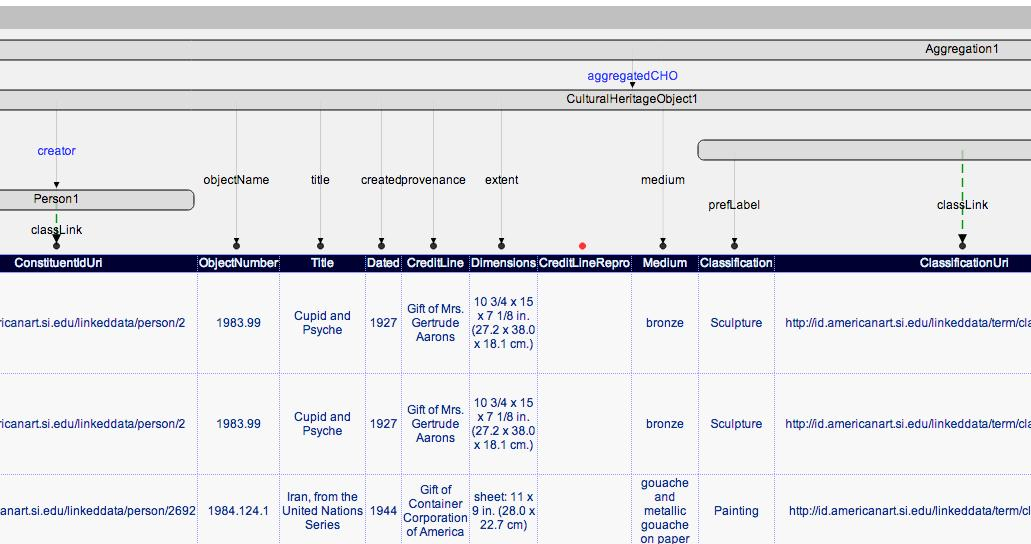
\includegraphics[width=\textwidth]{2-nozioni-preliminari/Immagini/karma-europeana.jpg}
	\caption{Karma Service Integration}\label{fig:karma-europeana}
\end{figure}

Karma è stato applicato con dati di diversa natura, spaziando dai musei ai dati di tipo bioinformatico. 
Nel caso dei dati di reperti dei musei, utilizzando questo tool si sono convertiti oltre 40000 reperti appartenenti alle collezioni dei musei seguendo l'\emph{Europeana Data Model}\footnote{Europeana Data Model: \url{http://pro.europeana.eu/page/edm-documentation}}, un modello di classificazione per le collezioni artistiche. A partire dai dati provenienti da diverse tabelle di un database SQL Server è stato possibile creare un nuovo dataset omogeneo secondo un nuovo modello dati. 

\subsection*{Peudom}

PEUDOM \cite{Cappiello:2015:UAE:2788341.2735632} è un progetto di ricerca sui mashup nato all'interno del dipartimento di Ingegneria Informatica del Politecnico di Milano. Si tratta di una piattaforma per la creazione di mashup interamente visuale che consente all'utente finale di sviluppare la propria applicazione su misura. La piattaforma guida l'utente nella scelta dei componenti e nelle definizioni delle relazioni, permettendo alcune operazioni e negandone altre secondo determinate regole di compatibilità definite a priori.
L'elemento peculiare di questa piattaforma è l'utilizzo di paradigmi di composizione visuale per definire la l'integrazione dei componenti a livello di presentazione. Questi paradigmi agiscono direttamente sull'interfaccia utente del mashup, in una sorta di programmazione in tempo reale nella quale i risultati della composizione sono visibili appena definiti.
Esistono due tipologie di componenti:

\begin{enumerate}
	\item \textbf{Wrapped UI Components}
	Questi sono i widget già predisposti da sviluppatori esperti, che specificano la logica dei i wrapper per l'accesso ai servizi Web e alle API
	\item \textbf{VI Components}
	VI Components significa \emph{Visual Integration based Component}s e si tratta di componenti creati direttamente dall'utente, manipolando i result set estratti da uno o più \emph{data component} e utilizzando i diversi UI template a disposizione
\end{enumerate}

Alla fine del processo di definizione dei componenti, questi vengono sincronizzati tra loro attraverso regole di sincronizzazione, che ne determinano il comportamento del mashup finale.

\begin{figure}[ht]
	\centering
	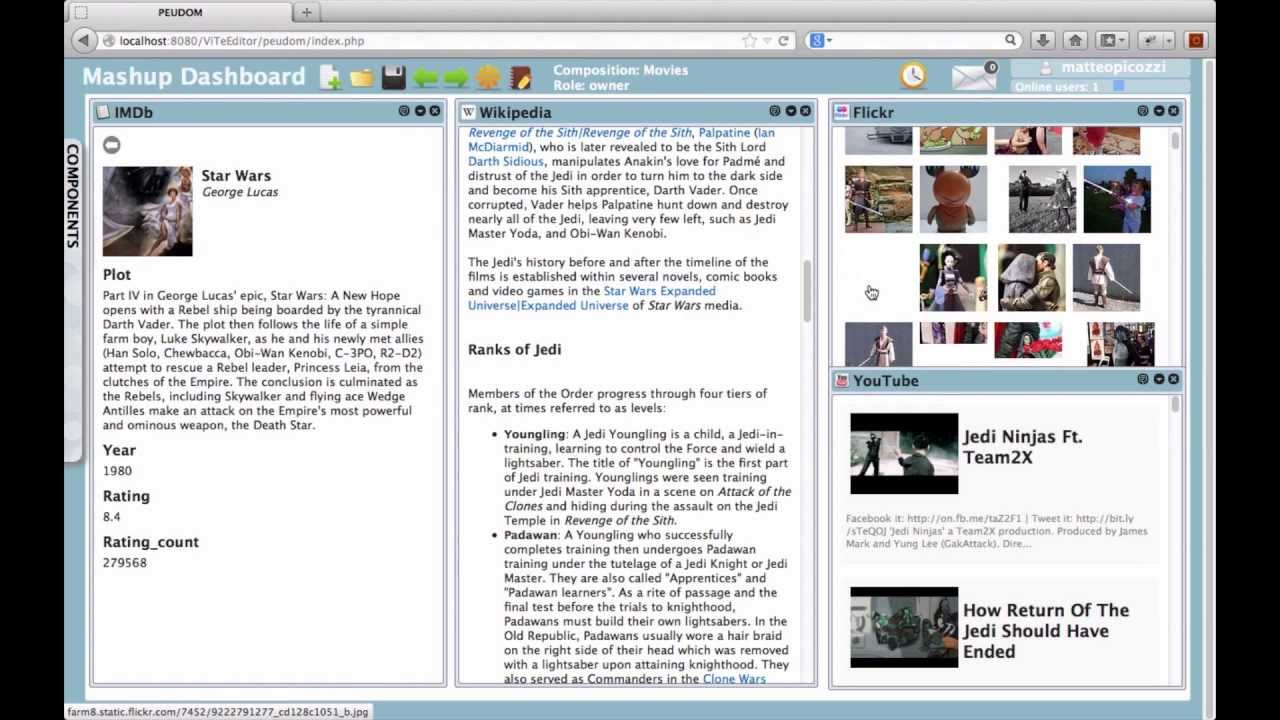
\includegraphics[width=\textwidth]{2-nozioni-preliminari/Immagini/peudom.jpg}
	\caption{Peudom}\label{fig:peudom}
\end{figure}

Nell'esempio in Figura \ref{fig:peudom} viene illustrata una \emph{Dashboard} dove è possibile creare i mashup specificando le fonti dalle quali acquisirli in modo da mostrarli nella stessa pagina. In questo caso si considerano dati di film ed è stato selezionato il film di \emph{Star Wars Parte IV}. Associati ai dati sul film estratti da IMDb è stato scelto di mostrare altri dati correlati al film provenienti da Wikipedia, Flickr e YouTube.

\subsection*{ADaPT}

ADaPT \cite{6816749_ADaPT} (Automatic Data Personalization and Tailoring) è un progetto sviluppato all'interno del Politecnico di Milano, che propone un framework per personalizzare l'accesso ai dati a partire dal contesto nel quale si trova l'utente. 

Dopo una fase di apprendimento delle abitudini dell'utente, l'applicazione è in grado di fornire le informazioni corrette quando si ripresenta lo stesso.
L'architettura presentata è formata da due componenti: il client e il server.
Il client è implementato in Android e utilizza il database interno SQLite e le connessioni con il server mediante TCP. Questo permette di utilizzare l'applicazione anche in condizioni di assenza di rete, perché i dati rilevanti vengono salvati anche nel database locale. La visualizzazione dei dati utilizzata è di tipo \emph{master-detail}, %global detail??
dove nella schermata principale è presentata la lista degli argomenti. Quando uno di essi è selezionato l'utente può esplorare i dati o cercare un elemento specifico con un filtro di ricerca per poi visualizzare i dati ricevuti nella pagina dei risultati. Una volta ottenuti, l'utente può visualizzare i dettagli dell'elemento desiderato in una nuova pagina. 

\subsection*{CADD}

CADD \cite{bolchini2007cadd} è un tool sviluppato all'interno del progetto Context-ADDICT del Politecnico di Milano, il cui scopo è la definizione di un framework che supporta l'integrazione di nuove informazioni basate sul contesto sui dispositivi mobili degli utenti. In particolare CADD è lo strumento che permette di progettare i contesti. In questo sistema è stato usato come modello di contesto il Context Dimension Tree (CDT), usato anche in CAMUS.  Una volta stabilito il modello di contesto, vengono creati i contesti dal designer, il quale viene guidato nell'associazione dei contenuti con la porzione di dati presente sul dispositivo mobile dell'utente finale. Come risultato, il sistema genera le query necessarie a selezionare i dati rilevanti per ogni contesto, in questo caso tramite espressioni XQuery\footnote{XQuery: \url{https://www.w3.org/TR/xquery/}} usate per potare i dati XML da inviare ai dispositivi mobili.
Il Context-ADDICT Server supporta la selezione dei dati online e l'invio dei risultati all'applicazione mobile. 

\begin{figure}[ht]
	\centering
	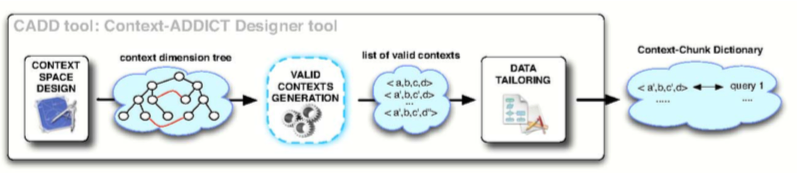
\includegraphics[width=\textwidth]{2-nozioni-preliminari/Immagini/cadd.png}
	\caption[CADD]{CADD (Fonte: \virgolette{CADD: a tool for context modeling and data tailoring}, 2007)}\label{fig:cadd}
\end{figure}

I componenti di CADD , come si può osservare in Figura  \ref{fig:cadd}, sono i seguenti:

\begin{itemize}
	\item \textbf{Context Space Designer Assistant}
	Il designer viene supportato nella modifica del CDT usando una procedura guidata. In questo modo può aggiungere, modificare ed eliminare i nodi dell'albero di contesto in modo semplice
	\item \textbf{Valid Contexts Generation}
	Una volta terminata la fase di design, questo componente genera automaticamente tutti i contesti validi, come combinazione dei valori dimensione
	\item \textbf{Data Tailoring Assistant}
	Il designer associa ogni contesto con la porzione corrispondente di dati disponibili. Questa associazione è svolta utilizzando uno schema globale di tipo ER. Basandosi sull'interazione con una rappresentazione grafica dello schema, il tool è in grado di generare una o più espressioni XQuery in modo da costruire le view corrispondenti ai dati
\end{itemize}